
\graphicspath{{./_figures/02_preliminaries/}}

\section{Notation and general results}\label{section:notation}
In this section we specify the notation used in this monograph and we point out some general results.

% Classical Logic Operators
For classical logic operations of conjunction, disjunction, negation and implication we write $\wedge$, $\vee$, $\neg$ and $\to$, respectively. 

% Crisp Sets
Let $A$ and $B$ be sets, we denote by $A \subseteq B$  when $A$ is a subset of $B$ where $A=B$ is possible; by $A \subsetneq B$ when $A$ is a proper subset of $B$; and by $A \not \subseteq B$ when $A$ is not a subset of $B$. The union, intersection, difference and Cartesian product of two sets $A$ and $B$ are denoted by $A \cup B$, $A \cap B$, $A \setminus B$ and $A \times B$, respectively. The cardinality and power set of a set $A$ are denoted by $|A|$ and $\mathcal{P}(A)$, respectively. The empty set is denoted by $\emptyset$. The complement of a subset $A \subseteq X$ is denoted by $A^c$. Given a topology on a set $A$, the topological closure, boundary and interior of $A$ are denoted by $\overline{A}$, $\partial A$, $\mathring A$, respectively.  We define $\mathbbm{1}_A : A \to \{0,1\}$ as the characteristic function of a set $A$, i.e., 
$$
\mathbbm{1}_A(x) = \left\{ \begin{array}{ll}
	1 &  \text{if }  x \in A, \\
	0 & \text{if }  x \not \in A.
\end{array}
\right.
$$
The symbol $\mathbb{N}$ denotes the set of positive integers, $\mathbb{Z}$ denotes the set of all integers, $\mathbb{R}$ denotes the set of all real numbers, and $\mathbb{N}_0 = \mathbb{N} \cup \{0\}$.

% Real sequences
A sequence of elements of a set $X$ is denoted by $\displaystyle \{a_n\}_{n \in A}$ with $A \subseteq \NN_0$ or, if $|A|$ is finite, by $\displaystyle \{a_n\}_{n=n_0}^{n_1}$ where $n$ goes from $n=n_0$ to $n=n_1$ with $n_0,n_1 \in \NN_0$.

% Functions
If $f: X \to Y$ is a function, then the domain of $f$ is denoted by $\Dom f$ and the range of $f$, i.e., the set $\{f(x) \mid x \in X\}$, is denoted by $\Ran f$. Let $A \subseteq X$ and $B \subseteq Y$, the image $f(A)$ and the preimage $f^{-1}(B)$ are defined by
$$f(A)=\{f(x) \mid x \in A\}, \quad f^{-1}(B) = \{x \in X \mid f(x) \in B\}.$$
The identity function is denoted by $\text{id}_X : X \to X$ and defined as $\text{id}_X(x)=x$ for all $x \in X$. If $A$ is a subset of $X$, then the restriction of $f$ to $A$ is defined as $\restr{f}{A} = f \circ \text{id}_A$. The composition of two functions $f : X \to Y$ and $g: U \to V$ with $Y \subseteq U$ is denoted by $g \circ f: X \to V$ and defined as $g \circ f(x)=g(f(x))$ for all $x \in X$. If a function $f: X \to Y$ is bijective then $f^{-1}: Y \to X$ denotes its inverse function and it satisfies $f^{-1}\circ f = \text{id}_X$ and  $f \circ f^{-1} = \text{id}_Y$.

% Common real functions
The floor and ceiling functions of real numbers are denoted by $\lfloor x \rfloor$ and $\lceil x \rceil$ for all $x \in \RR$, respectively. The absolute value of a real number $x \in \RR$ is denoted by $|x|$. The natural logarithm (i.e., the logarithm with respect to $e$) is denoted by $\ln(x)$ for all $x \in (0,+\infty)$, whereas the logarithm with respect to $\lambda \in (0,1) \cup (1,+\infty)$ is denoted by $\log_{\lambda}(x)$ for all $x \in (0,+\infty)$.

% Side limits
If $f:X \to \RR$ is a real function then for $a,b \in X$ the values $f(a^+)$ and $f(b^{-})$ denote the right and left-hand limits of $f$ in the points $a$ and $b$, respectively, i.e.,
$$f(a^+)= \lim_{x \to a^{+}} f(x), \quad f(b^{-})= \lim_{x \to b^{-}} f(x).$$

% Unary and Binary Operations
We denote as unary functions those that take one argument, and as binary functions those that take two arguments. Let us consider a binary function $F: X \times Y \to Z$ where $X,Y,Z \subseteq \RR$. Then, for each fixed $x_0 \in X$ the vertical section of $F$ is denoted by $F(x_0,\cdot)$. Similarly, for each fixed $y_0 \in Y$ the horizontal section of $F$ is denoted by $F(\cdot,y_0)$. These functions are defined as follows
\begin{center}
\noindent\begin{minipage}{.35\linewidth}
\begin{align*}
	F(x_0,\cdot) \colon Y & \longrightarrow Z \\[-1ex]
	y & \longmapsto F(x_0,y),
\end{align*}
\end{minipage}%
\begin{minipage}{.35\linewidth}
\begin{align*}
	F(\cdot,y_0) \colon X & \longrightarrow Z \\[-1ex]
	x & \longmapsto F(x,y_0).
\end{align*}
\end{minipage}
\end{center}

% Real Intervals
To denote a closed interval of \RR we write $[a,b]$, for an open interval $(a,b)$ and for half-open intervals $[a,b)$ or $(a,b]$. Further, we use a vertical line at the beginning or at the end of an interval to indicate that this extreme can be considered either open or closed. More specifically, if $a,b \in \mathbb{R}$ with $a<b$, then $[a,b|$ can be either $[a,b)$ or $[a,b]$ and $|a,b|$ can be either $[a,b)$, $[a,b]$, $(a,b]$ or $(a,b)$. In particular, this notation is used to simplify the number of cases in some results, in which there appear functions with one or more jump discontinuities that can either be left or right-continuous in some discontinuity points. For instance, if we consider a function $f:\mathbb{R} \to [0,1]$ given by
$$
f(x)
=\left\{ \begin{array}{ll}
	1 & \text{if } x\in [a,b|,\\
	0 &   \text{otherwise},
\end{array}
\right.
$$
we say that we are considering two types of functions, one with $f(x)=1$ if $x \in[a,b]$ and 0 otherwise, and another with $f(x)=1$ if $x \in[a,b)$ and 0 otherwise. That is to say, we consider the functions with $f(x)=1$ for all $x \in [a,b)$, $f(x)=0$ for all $x \in \mathbb{R} \setminus [a,b]$ and $f(b)\in \{0,1\}$, i.e.,  $f$ can either be left or right-continuous on $x=b$. 

% Extended real line
The extended real line $\RR \cup \{-\infty,+\infty\}$ is denoted by $[-\infty,+\infty]$ and the set $I \times I$ where $I$ is an interval, is denoted by $I^2$. The conventions when arithmetic operations are done on $+\infty$, $-\infty$ and 0 (e.g., the value of the symbols $0 \cdot (+\infty)$, $+\infty+(-\infty)$ or $\frac{0}{0}$) depend on the context and they are specified when applicable.

%Iterates of a Function
The iterates $f^{n}(x)$ of a function $f$ with $\Dom f = X$ and $\Ima f \subseteq X$ are defined recursively as follows
$$f^{0}(x)=x, \quad f^{n+1}(x)=f(f^n(x)), \quad \text{for all } x \in X, n \in \NN_0.$$
If the function $f$ is invertible, then the iterates of $f$ can also be defined for negative indices
$$f^{n-1}(x) = f^{-1}(f^{n}(x)), \quad \text{for all } x \in X, n \in \ZZ \setminus \NN.$$

% Power notation of Associative Operators
We say that a binary function $F:[a,b]^2 \to [a,b]$ with $a,b \in \RR$ is an associative operator with neutral element $e \in [a,b]$ if $F(x,F(y,z))=F(F(x,y),z)$ for all $x,y,z \in [a,b]$ and $F(x,e)=F(e,x)=x$ for all $x \in [a,b$]. In this case, the power notation $x_{F}^{(n)}$ where $n \in \mathbb{N}_0$ is defined recursively as follows 
\begin{equation}\label{eq:powers:genF}
x_{F}^{(n)}= 
\left\{ \begin{array}{ll}
	e &  \text{if } n=0, \\
	x & \text{if }  n=1,\\
	F(x,x_{F}^{(n-1)}) &  \text{if }  n>1.
\end{array}
\right.
\end{equation}

The following result simplifies the study of the continuity of binary functions $F:[0,1]^2 \to [0,1]$.

\begin{theorem}[\bf{\cite[Theorem A.0.4]{Klement2000}}]\label{theorem:A04}
	For a function $F:[0,1]^2 \to [0,1]$ which is monotonic with respect to one variable the following statements are equivalent:
	\begin{enumerate}[label=(\roman*)]
		\item $F$ is continuous.
		\item $F$ is continuous in each variable.
	\end{enumerate}
\end{theorem}

% Phi-Conjugates
By $\Phi$ we denote the family of all increasing bijections from $[0,1]$ to $[0,1]$. The conjugacy of two functions with respect to this set of functions is defined as follows.
\begin{definition}[\bf{\cite{Baczynski2008}}]
Two functions $f,g: [0,1]^n \to [0,1]$ are said to be $\Phi$-conjugate if there exists $\varphi \in \Phi$ such that $g=f_{\varphi}$ where
$$f_{\varphi}(x_1,\dots,x_n) = \varphi^{-1}(f(\varphi(x_1),\dots,\varphi(x_n))), \quad \text{for all } (x_1,\dots,x_n) \in [0,1]^n.$$
\end{definition}

% Pseudo-Inverses
In order to define a function that acts similarly to an inverse but for non-bijective functions, the concept of pseudo-inverse of monotone functions is considered.
\begin{definition}[\bf{\cite[Definition 3.2]{Klement2000}}]\label{pseudo-inverse} Let $[a,b]$ and $[c,d]$ be two closed subintervals of the extended real line $[-\infty,+\infty]$ and let $f:[a,b] \rightarrow [c,d]$ be a monotone function. Then the \emph{pseudo-inverse} $f^{(-1)}:[c,d] \rightarrow [a,b]$ is defined by
	$$f^{(-1)}(y)=\sup\{ x \in [a,b] \mid (f(x)-y)(f(b)-f(a)) <0 \}.$$
\end{definition}
If we distinguish the cases when $f$ is increasing, decreasing or a constant function in Definition \ref{pseudo-inverse}, a simpler expression for its pseudo-inverse can be obtained. In Figure \ref{fig:pseudo-inverses} there is an example of two monotone functions with their corresponding pseudo-inverses.
\begin{corollary}[\bf{\cite[Corollary 3.3]{Klement2000}}]\label{cor:pseudo-inverse}
Let $f:[a,b] \rightarrow [c,d]$ be a monotone function, where $[a,b]$ and $[c,d]$ are closed subintervals of the extended real line $[-\infty,+\infty]$.
\begin{enumerate}[label=(\roman*)]
		\item If $f(a) < f(b)$, i.e., if $f$ is increasing and non-constant, then for all $y \in [c,d]$ we obtain the simpler formula
		$$f^{(-1)}(y) = \sup \{ x \in [a,b] \mid f(x)<y \}.$$
		Moreover, the function $f^{(-1)}$ is increasing and left-continuous, and for each $y \in [c,f(a)]$ we have $f^{(-1)}(y)=a$, and for each $ y \in (f(b),d]$ we get $f^{(-1)}(y)=b$. Also, $(f^{(-1)})^{(-1)}=f$ if and only if $f$ is left-continuous and $f(a)=c$.
		\item If $f(a)>f(b)$, i.e., if $f$ is decreasing and non-constant, then for all $y \in [c,d]$ we obtain the simpler formula
		$$f^{(-1)}(y)= \sup \{ x \in [a,b] \mid f(x)>y \}.$$
		Moreover, the function $f^{(-1)}$ is decreasing and right-continuous, and for each $y \in [c,f(b)]$ we have $f^{(-1)}(y)=b$, and for each $y \in [f(a),d]$ we get $f^{(-1)}(y)=a$. Also, $(f^{(-1)})^{(-1)}=f$ if and only if $f$ is right-continuous and $f(b)=c$.
		\item If $f(a)=f(b)$, i.e., if $f$ is a constant function, then for all $y \in [c,d]$ we have $f^{(-1)}(y)=a$.
	\end{enumerate}
\end{corollary}

\begin{figure}
\centering
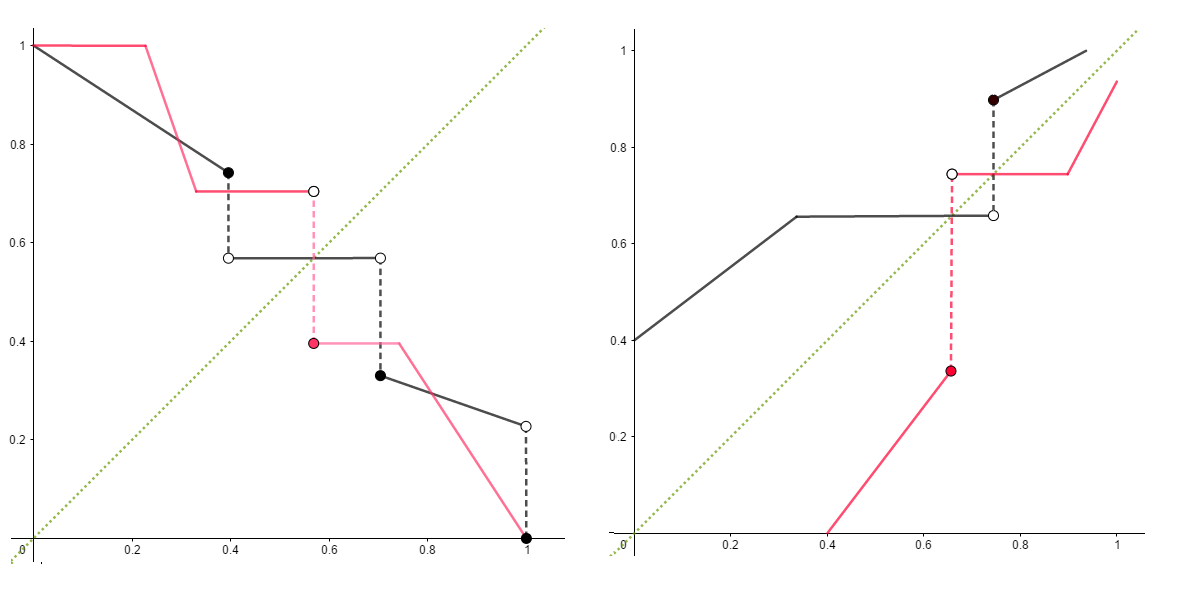
\includegraphics[scale=0.4]{pseudo-inverses.png}
\caption{A decreasing function (left) and increasing function (right) together with their respective pseudo-inverses (pink graphs).}\label{fig:pseudo-inverses}
\end{figure}


Some basic properties of the pseudo-inverse of a monotone function are recalled in the following proposition.

\begin{proposition}[\bf{\cite[Remark 3.4]{Klement2000}}]\label{prop:pseudo-inverse}
Let $f:[a,b] \rightarrow [c,d]$ be a monotone function, where $[a,b]$ and $[c,d]$ are closed subintervals of the extended real line $[-\infty,+\infty]$, and let $f^{(-1)}$ be its pseudo-inverse.
	\begin{enumerate}[label=(\roman*)]
		\item  The pseudo inverse $f^{(-1)}$ of $f$ coincides with the inverse function $f^{-1}$ of $f$ if and only if $f$ is a bijection.
		\item The pseudo inverse $f^{(-1)}$ of $f$ is continuous if and only if $f$ is strictly monotone on the set $f^{(-1)}([c,d))$.
		\item $f^{(-1)} \circ f \leq \text{id}_{[a,b]}$.
		\item The equality $f \circ f^{(-1)} \circ f = f$ holds if and only if $\displaystyle f(x_0)=\lim_{x \to x_0^{+}} f(x)$ whenever there are numbers $x_0 \in [a,b]$ and $\varepsilon >0$ such that the restriction $f\mid_{(x_0,x_0+\varepsilon]}$ is a constant function.
		\item If $f$ is strictly monotone then the restriction of $f^{(-1)}$ to Ran$(f)$, i.e., the function $f^{(-1)}\mid_{\text{Ran}(f)} : \text{Ran}(f) \rightarrow [a,b]$, is also strictly monotone. Moreover, in this case we have the following identities:
		$$ f \circ f^{(-1)} \mid_{\text{Ran}(f)} = \text{id}_{\text{Ran}(f)},$$
		$$f^{(-1)} \circ f = \text{id}_{[a,b]}.$$
		\item If $f$ is surjective then we have that $f \circ f^{(-1)} = \text{id}_{[c,d]}$.
		\item If $\varphi:[a,b] \rightarrow [a,b]$ and $\psi : [c,d] \rightarrow [c,d]$ are monotone bijections then
		$$(f \circ \varphi)^{(-1)} = \varphi^{-1} \circ f^{(-1)},$$
		$$(\psi \circ f)^{(-1)} = f^{(-1)} \circ \psi^{-1}.$$
	\end{enumerate}
\end{proposition}

Let us anticipate that some results of this monograph involve increasing functions $g:(0,1)\to [0,1]$ which are idempotent in its image except for 0 and 1. Although in the corresponding result we outline such condition by indicating that $g(z)=z$ for all $z \in \Ima g \setminus \{0,1\}$, it is easy to prove that this kind of functions are characterized by the following result.
\begin{lemma}\label{lem:idempotentfunctions} Let $g:(0,1) \to [0,1]$ be an increasing function. Then $g(z)=z$ for all $z \in \Ima g \setminus \{0,1\}$ if and only if in the interval in which $g$ is not 0 or 1, $g$ is the identity function, except for a countable set of intervals (open or closed or half-open) on which it is instead constant, taking a value which falls inside that interval.
\end{lemma}
\begin{proof}
	Let $g :(0,1) \to [0,1]$ be an increasing function. First, let us suppose that for every $z \in \Ima g \setminus \{0,1\}$ we have that $g(z)=z$. Now, consider that there exists a $y_0\in(0,1)$ such that $y_0<g(y_0)$ with $g(y_0)\in(0,1)$. Then, for all $y\in[y_0,g(y_0)]$ we have that
	$$y_0 \leq y \leq g(y_0) \Rightarrow g(y_0) \leq g(y) \leq g(g(y_0)) \Rightarrow g(y_0) \leq g(y) \leq  g(y_0) \Rightarrow g(y)=g(y_0),$$
	and we obtain that $g(y)=g(y_0)$ for all $y \in [y_0,g(y_0)]$. Analogously, it can be proved that if there exists a $y_0\in(0,1)$ such that $y_0>g(y_0)$ with $g(y_0)\in(0,1)$, then $g(y)=g(y_0)$ for all $y\in[g(y_0),y_0]$.  Thus, when we consider $y \in (0,1)$ with $g(y) \in (0,1)$ and $y \not = g(y)$, then $g(y)$ lies in an interval where $g$ is constant, taking a value which falls inside that interval. Therefore, the result follows since in this case, $g$ is the identity function, interrupted by up to countably many intervals on which $g$ is constant, taking a value which falls inside that interval.  For the reverse implication, it is straightforward to verify that if $g$ is the kind of function described above, then it is idempotent in its image except for 0 or 1.
\end{proof}
\begin{example} Some examples of increasing functions $g:(0,1) \to [0,1]$ which are idempotent in its image except for 0 and 1 are the following:
	$$ g_1(x)=x, 
	\quad 
	g_2(x)= \left\{ \begin{array}{ll}
		0 &  \text{if }  x \in \left(0,\frac{1}{4}\right), \\[3pt]
		x & \text{if }  x \in \left[\frac{1}{4},\frac{3}{4}\right],\\[3pt]
		1 &  \text{if }  x \in \left(\frac{3}{4},1\right),
	\end{array}
	\right.
	$$
	$$
	g_3(x)= \left\{ \begin{array}{ll}
		\frac{1}{4} &  \text{if }  x \in \left(0,\frac{1}{2}\right), \\[3pt]
		\frac{1}{2} & \text{if }  x \in \left[\frac{1}{2},\frac{3}{4}\right],\\[3pt]
		x &  \text{if }  x \in \left(\frac{3}{4},1\right),
	\end{array}
	\right.
	\quad
	g_4(x)= \sum_{k \geq 1} \frac{1}{2^k} \mathbbm{1}_{\left[\frac{1}{2^k},\frac{1}{2^{k-1}}\right)}(x).
	$$
\end{example}

\section{Fuzzy sets, membership functions and linguistic variables}

In this section we only provide the definitions of fuzzy set, membership function, linguistic variable and fuzzy partition. For deeper information about these concepts there are many books devoted to this topic, see for instance \cite{Cox1994,Klir1995,Zimmermann1991,Nguyen2018}.

A fuzzy set is a set whose elements have degrees of membership, and they are an extension of the classical notion of set, known as crisp set.
\begin{definition}[\bf{\cite{Zadeh1965}}]\label{def:fuzzyset}
	Let $X$ be a classical set of objects, called the \emph{universe}. A \emph{fuzzy set} $A$ of $X$ is characterized by a function $\mu_A: X \to [0,1]$, which is called the \emph{membership function} of $A$. For all $x \in X$,  the value $\mu_A(x)$ indicates the \emph{degree of membership} of $x$ in the fuzzy set $A$.
\end{definition}

The \textit{core} and \textit{support} of a fuzzy set $A$ of $X$ with membership function $\mu_A$ are defined as $C(A)= \{ x \in X \mid \mu_A(x)=1\}$ and $S(A)= \{x \in X \mid \mu_A(x)>0\}$, respectively.

In the literature, several structures of membership functions for the construction of fuzzy sets have been considered. The choice of these functions depends on the particular problem and/or application \cite{Mitaim1996}. In Example \ref{ex:mem_fun} some of the most well-known structures of membership functions are recalled.

\begin{example}\label{ex:mem_fun}
Let the universe $X$ be the set of real numbers \RR.
	\begin{itemize}
		\item Let $a \in \RR$, the corresponding \emph{singleton membership function} is defined by
		$$
		\mu_{singleton}(x;a)= \left\{ \begin{array}{ll}
			1 &  \text{if }  x =a, \\
			0 & \text{otherwise}.
		\end{array}
		\right.
		$$
		\item Let $a,b,c \in \RR$ with $a<b<c$, the corresponding \emph{triangular membership function} is defined by
		$$
		\mu_{triangular}(x;a,b,c)= \left\{ \begin{array}{ll}
			0 &  \text{if }  x \leq a, \\[3pt]
			\frac{x-a}{b-a} & \text{if }  a < x \leq b,\\[3pt]
			\frac{c-x}{c-b} &  \text{if }  b < x \leq c, \\[3pt]
			0 &  \text{if } x \geq c.
		\end{array}
		\right.
		$$
		\item Let $a,b,c,d \in \RR$ with $a<b<c<d$, the corresponding \emph{trapezoidal membership function} is defined by
				$$
		\mu_{trapezoidal}(x;a,b,c,d)= \left\{ \begin{array}{ll}
			0 &  \text{if }  x \leq a, \\[3pt]
			\frac{x-a}{b-a} & \text{if }  a < x \leq b,\\[3pt]
			1 & \text{if } b < x \leq c, \\[3pt]
			\frac{d-x}{d-c} &  \text{if }  c < x \leq d, \\[3pt]
			0 &  \text{if } x \geq d.
		\end{array}
		\right.
		$$
		\item Let $\mu, \sigma \in \RR$, the corresponding \emph{Gaussian membership function} is defined by
		$$
		\mu_{gaussian}(x;\mu,\sigma)= e^{-\frac{1}{2} \left(\frac{(x-\mu)}{\sigma}\right)^2}.
		$$
	\end{itemize}
\end{example}

A linguistic variable is a variable whose values are words or sentences in a natural or artificial language.
\begin{definition}[\bf{\cite{Zadeh1975}}]\label{def:fuzzyvariable}
	A \emph{linguistic variable} is characterized by a quintuple \linebreak $(X,T(X),U,G,\mu)$, where $X$ is the name of the variable; $T(X)$ is the set of linguistic terms of $X$; $U$ is a set called the universe of discourse; $G$ is the syntactic rule that generates the terms of $T(X)$; and $\mu$ is a semantic rule that associates the meaning with each linguistic value $X$, where $\mu(X)$ denotes a fuzzy set of $U$. For a given $X$, the name generated by $G$ is called \emph{linguistic term}.
\end{definition}
% Fuzzy partition

A fuzzy partition can be generally defined as a finite collection of fuzzy sets.  Depending on the additional conditions imposed on the fuzzy sets, different types of fuzzy partitions have been defined \cite{Bezdek1978,Dumitrescu1992,Ovchinnikov1991}. For instance, a widely-used type of fuzzy partition for real, closed intervals are Ruspini partitions.

\begin{definition}[\bf{\cite[Definition 1]{Perfilieva2006}}]
	Let $x_1 < \dots < x_n$ be fixed nodes within $[a,b]$ such that $x_1=a$, $x_n=b$ and $n \geq 2$. We say that the fuzzy sets $A_1, \dots, A_n$ establish a \emph{Ruspini partition} of $[a,b]$ if they fulfill the following conditions:
	\begin{itemize}
		\item $\mu_{A_k}: [a,b] \to [0,1]$, $\mu_{A_k}(x_k)=1$ for all $k \in \{1,\dots,n\}$;
		\item $\mu_{A_k}(x)=0$ if $x \not \in (x_{k-1},x_{k+1})$ for all $k \in \{1,\dots,n\}$, where for uniformity of notation, we set $x_0=a$ and $x_{n+1}=b$;
		\item $\mu_{A_k}$ is continuous for all $k \in \{1,\dots,n\}$;
		\item If $k \in \{2,\dots,n\}$ then $\mu_{A_k}(x)$ is strictly increasing on $[x_{k-1},x_k]$;
		\item If $k \in \{1,\dots,n-1\}$ then $\mu_{A_k}(x)$ is strictly decreasing on $[x_k,x_{k+1}]$;
		\item $\displaystyle \sum_{k=1}^n \mu_{A_k}(x)=1$, for all $x \in [a,b]$.
 	\end{itemize}
\end{definition}

In practical terms, for each linguistic variable involved in a concrete problem usually a fuzzy partition of its domain is considered (see Figure \ref{fig:example_linguistic_label}).

\begin{figure}[H]
	\centering
\tikzset{every picture/.style={line width=0.75pt}} %set default line width to 0.75pt        

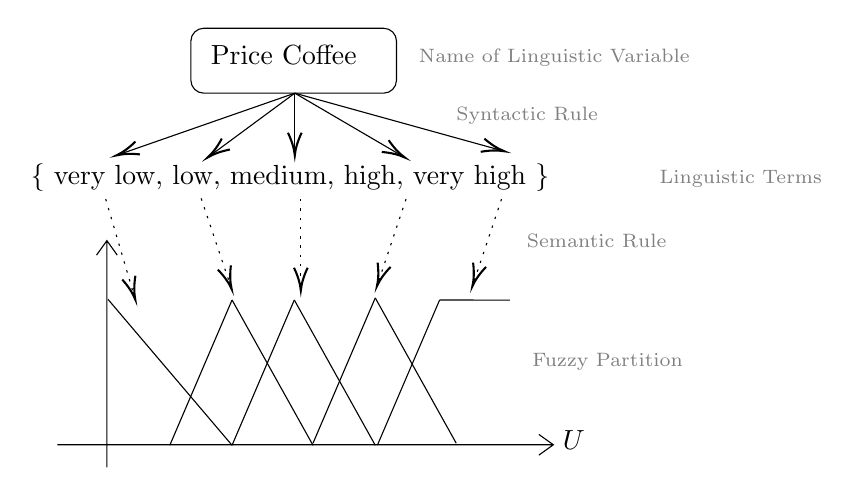
\begin{tikzpicture}[x=0.75pt,y=0.75pt,yscale=-1,xscale=1]
	%uncomment if require: \path (0,300); %set diagram left start at 0, and has height of 300
	
	%Rounded Rect [id:dp5043193231595386] 
	\draw   (220.35,26.26) .. controls (220.35,22.8) and (223.15,20) .. (226.61,20) -- (313.17,20) .. controls (316.63,20) and (319.43,22.8) .. (319.43,26.26) -- (319.43,45.03) .. controls (319.43,48.48) and (316.63,51.29) .. (313.17,51.29) -- (226.61,51.29) .. controls (223.15,51.29) and (220.35,48.48) .. (220.35,45.03) -- cycle ;
	
	%Straight Lines [id:da7800093448947967] 
	\draw    (270.43,51.29) -- (186.32,80.63) ;
	\draw [shift={(184.43,81.29)}, rotate = 340.77] [color={rgb, 255:red, 0; green, 0; blue, 0 }  ][line width=0.75]    (10.93,-3.29) .. controls (6.95,-1.4) and (3.31,-0.3) .. (0,0) .. controls (3.31,0.3) and (6.95,1.4) .. (10.93,3.29)   ;
	%Straight Lines [id:da4016471229943066] 
	\draw    (270.43,51.29) -- (230.04,81.1) ;
	\draw [shift={(228.43,82.29)}, rotate = 323.57] [color={rgb, 255:red, 0; green, 0; blue, 0 }  ][line width=0.75]    (10.93,-3.29) .. controls (6.95,-1.4) and (3.31,-0.3) .. (0,0) .. controls (3.31,0.3) and (6.95,1.4) .. (10.93,3.29)   ;
	%Straight Lines [id:da2825911929820748] 
	\draw    (270.43,51.29) -- (270.43,79.29) ;
	\draw [shift={(270.43,81.29)}, rotate = 270] [color={rgb, 255:red, 0; green, 0; blue, 0 }  ][line width=0.75]    (10.93,-3.29) .. controls (6.95,-1.4) and (3.31,-0.3) .. (0,0) .. controls (3.31,0.3) and (6.95,1.4) .. (10.93,3.29)   ;
	%Straight Lines [id:da9535710275229592] 
	\draw    (270.43,51.29) -- (321.7,81.28) ;
	\draw [shift={(323.43,82.29)}, rotate = 210.32] [color={rgb, 255:red, 0; green, 0; blue, 0 }  ][line width=0.75]    (10.93,-3.29) .. controls (6.95,-1.4) and (3.31,-0.3) .. (0,0) .. controls (3.31,0.3) and (6.95,1.4) .. (10.93,3.29)   ;
	%Straight Lines [id:da3867224952909125] 
	\draw    (270.43,51.29) -- (369.5,78.75) ;
	\draw [shift={(371.43,79.29)}, rotate = 195.49] [color={rgb, 255:red, 0; green, 0; blue, 0 }  ][line width=0.75]    (10.93,-3.29) .. controls (6.95,-1.4) and (3.31,-0.3) .. (0,0) .. controls (3.31,0.3) and (6.95,1.4) .. (10.93,3.29)   ;
	%Shape: Axis 2D [id:dp9498815687860906] 
	\draw  (156,220.69) -- (395,220.69)(179.9,122.33) -- (179.9,231.62) (388,215.69) -- (395,220.69) -- (388,225.69) (174.9,129.33) -- (179.9,122.33) -- (184.9,129.33)  ;
	%Straight Lines [id:da20391340899144117] 
	\draw    (180.43,150.62) -- (240.2,220.93) ;
	%Straight Lines [id:da5667233317973046] 
	\draw    (210.2,220.93) -- (240.2,150.93) ;
	%Straight Lines [id:da7732667640639663] 
	\draw    (279.2,220.93) -- (240.2,150.93) ;
	%Straight Lines [id:da7170851127463433] 
	\draw    (240.2,220.93) -- (270.2,150.93) ;
	%Straight Lines [id:da03498652326961316] 
	\draw    (309.2,220.93) -- (270.2,150.93) ;
	%Straight Lines [id:da8429969469846545] 
	\draw    (279.2,219.93) -- (309.2,149.93) ;
	%Straight Lines [id:da9649226998275144] 
	\draw    (348.2,219.93) -- (309.2,149.93) ;
	%Straight Lines [id:da42538415289147746] 
	\draw    (310.2,220.93) -- (340.2,150.93) ;
	%Straight Lines [id:da2789076103705388] 
	\draw    (374,151) -- (340.2,150.93) ;
	%Straight Lines [id:da17676732587924837] 
	\draw  [dash pattern={on 0.84pt off 2.51pt}]  (179.33,102.33) -- (192.99,148.75) ;
	\draw [shift={(193.56,150.67)}, rotate = 253.6] [color={rgb, 255:red, 0; green, 0; blue, 0 }  ][line width=0.75]    (10.93,-3.29) .. controls (6.95,-1.4) and (3.31,-0.3) .. (0,0) .. controls (3.31,0.3) and (6.95,1.4) .. (10.93,3.29)   ;
	%Straight Lines [id:da9172065472117523] 
	\draw  [dash pattern={on 0.84pt off 2.51pt}]  (225.33,102) -- (239.36,143.77) ;
	\draw [shift={(240,145.67)}, rotate = 251.43] [color={rgb, 255:red, 0; green, 0; blue, 0 }  ][line width=0.75]    (10.93,-3.29) .. controls (6.95,-1.4) and (3.31,-0.3) .. (0,0) .. controls (3.31,0.3) and (6.95,1.4) .. (10.93,3.29)   ;
	%Straight Lines [id:da20807959196798587] 
	\draw  [dash pattern={on 0.84pt off 2.51pt}]  (273.33,102.33) -- (273.33,144.33) ;
	\draw [shift={(273.33,146.33)}, rotate = 270] [color={rgb, 255:red, 0; green, 0; blue, 0 }  ][line width=0.75]    (10.93,-3.29) .. controls (6.95,-1.4) and (3.31,-0.3) .. (0,0) .. controls (3.31,0.3) and (6.95,1.4) .. (10.93,3.29)   ;
	%Straight Lines [id:da6557057175466074] 
	\draw  [dash pattern={on 0.84pt off 2.51pt}]  (324,102.33) -- (310.63,142.44) ;
	\draw [shift={(310,144.33)}, rotate = 288.43] [color={rgb, 255:red, 0; green, 0; blue, 0 }  ][line width=0.75]    (10.93,-3.29) .. controls (6.95,-1.4) and (3.31,-0.3) .. (0,0) .. controls (3.31,0.3) and (6.95,1.4) .. (10.93,3.29)   ;
	%Straight Lines [id:da5598108462458484] 
	\draw  [dash pattern={on 0.84pt off 2.51pt}]  (370,102.33) -- (356.63,142.44) ;
	\draw [shift={(356,144.33)}, rotate = 288.43] [color={rgb, 255:red, 0; green, 0; blue, 0 }  ][line width=0.75]    (10.93,-3.29) .. controls (6.95,-1.4) and (3.31,-0.3) .. (0,0) .. controls (3.31,0.3) and (6.95,1.4) .. (10.93,3.29)   ;
	
	% Text Node
	\draw (142,84) node [anchor=north west][inner sep=0.75pt]   [align=left] {\{ very low, low, medium, high, very high \}};
	% Text Node
	\draw (228.72,27.02) node [anchor=north west][inner sep=0.75pt]   [align=left] {Price Coffee};
	% Text Node
	\draw (329,29) node [anchor=north west][inner sep=0.75pt]  [font=\scriptsize,color={rgb, 255:red, 128; green, 128; blue, 128 }  ,opacity=1 ] [align=left] {Name of Linguistic Variable};
	% Text Node
	\draw (347,56.67) node [anchor=north west][inner sep=0.75pt]  [font=\scriptsize,color={rgb, 255:red, 128; green, 128; blue, 128 }  ,opacity=1 ] [align=left] {Syntactic Rule};
	% Text Node
	\draw (398.33,212.73) node [anchor=north west][inner sep=0.75pt]    {$U$};
	% Text Node
	\draw (445,87.33) node [anchor=north west][inner sep=0.75pt]  [font=\scriptsize,color={rgb, 255:red, 128; green, 128; blue, 128 }  ,opacity=1 ] [align=left] {Linguistic Terms};
	% Text Node
	\draw (381,118) node [anchor=north west][inner sep=0.75pt]  [font=\scriptsize,color={rgb, 255:red, 128; green, 128; blue, 128 }  ,opacity=1 ] [align=left] {Semantic Rule};
	% Text Node
	\draw (383.67,175.33) node [anchor=north west][inner sep=0.75pt]  [font=\scriptsize,color={rgb, 255:red, 128; green, 128; blue, 128 }  ,opacity=1 ] [align=left] {Fuzzy Partition};
\end{tikzpicture}
\caption{Conceptual example of a linguistic variable ``Price Coffee''.}\label{fig:example_linguistic_label}
\end{figure}
\section{Fuzzy negations, t-norms, t-conorms, uninorms and copulas}

In this section we introduce some of the main operators of fuzzy logic: fuzzy negations, t-norms, t-conorms, uninorms and copulas.

\subsection{Fuzzy negations}
A fuzzy negation $N$ is a generalization of the classical negation $\neg$, whose truth table is defined by the conditions: $\neg 0=1$ and $\neg 1 =0$.
\begin{definition}[\bf{\cite[Definition 1.1]{Fodor1994}}]\label{def:fuzzy_negation}
	A unary function $N:[0,1] \to [0,1]$ is said to be a \emph{fuzzy negation} if it satisfies:
	\begin{description}
		\item[(N1)] $N(0)=1$ and $N(1)=0$. \hfill (Boundary Condition)
		\item[(N2)] $N$ is decreasing. \hfill (Monotonicity)
	\end{description}
\end{definition}
In Definition \ref{def:fuzzy_negation}, the property {\bf (N1)} imposes the boundary conditions of the classical negation and {\bf (N2)} points out that as the belongingness of an element to one set increases, its belongingness to the complement set decreases. Since the definition of a fuzzy negation is wide, other restrictions on this kind of functions have been introduced in the literature.
\begin{definition}[\bf{\cite{Fodor1994}}] A fuzzy negation $N$ is called
	\begin{enumerate}[label=(\roman*)]
		\item  \emph{strict} if it satisfies:
		\begin{description}
			\item[(N3)] $N$ is strictly decreasing.
			\item[(N4)] $N$ is continuous.
		\end{description}
		\item \emph{strong} if it is an involution, i.e., if it satisfies:
		\begin{description}
			\item[(N5)] $N(N(x))=x$ for all $x \in [0,1]$.
		\end{description}
		\item \emph{non-vanishing} if ($N(x)=0 \Leftrightarrow x=1$).
		\item \emph{non-filling} if ($N(x)=1 \Leftrightarrow x=0$).
	\end{enumerate}
\end{definition}

\begin{corollary}[\bf{\cite[Corollary 1.4.6]{Baczynski2008}}]
	Every strong fuzzy negation is strict. Every strict negation is non-vanishing and non-filling.
\end{corollary}

In Table \ref{table:fuzzy_negations} examples of well-known fuzzy negations can be found. Moreover, in Figure \ref{fig:sugeno_negation} there is the plot of some fuzzy negations in the Sugeno class for different values of $\lambda$.
\begin{table}[ht!]
	\setlength\tabcolsep{5pt}
	\renewcommand{\arraystretch}{1.5}
	\centering
	\begin{tabular}{|c|l|l|} \hline
		\bf Name & \multicolumn{1}{|c|}{\bf Formula} & \multicolumn{1}{|c|}{\bf Properties} \\[2pt]  
		\hline \bf Classic & $\NC(x)=1-x$ & strong \\[2pt] 
		\hline \bf G\"odel negation  & $\NDOne(x)=\left\{\begin{array}{ll}1&\hbox{if } x=0\\0&\hbox{if } x\in(0,1]\end{array}\right.$ & non-filling\\[2pt] 
		\hline \bf Greatest & $\NDTwo(x)=\left\{\begin{array}{ll}1&\hbox{if } x\in[0,1)\\0&\hbox{if } x=1\end{array}\right.$ & non-vanishing  \\[2pt] 
		\hline - & $N_{\bf K}(x)=1-x^2$ & strict  \\[2pt] 
		\hline - & $N_{\bf R}(x)=1-\sqrt{x}$ & strict  \\[2pt] 
		\hline \bf Sugeno class & $N^{\lambda}(x)=\frac{1-x}{1-\lambda x}, \quad \lambda \in (-\infty,1)$ & strong  \\[2pt] 
		\hline \bf Yager class & $N^{w}(x)=(1-x^w)^{\frac{1}{w}}, \quad w \in (0,+\infty)$ & strong  \\
		\hline
	\end{tabular}
	\caption{Basic Fuzzy Negations.}\label{table:fuzzy_negations}
\end{table}

\begin{figure}[ht!]
	\centering
	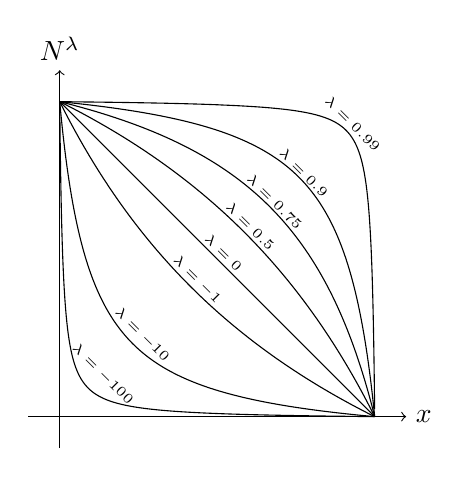
\begin{tikzpicture}
		\draw[scale=4,->] (-0.1, 0) -- (1.1, 0) node[right] {$x$};
		\draw[scale=4,->] (0, -0.1) -- (0, 1.1) node[above] {$N^{\lambda}$};
		\node at (0.4,0.4) [above,rotate=-45]  {\tiny $\lambda=-100$};
		\node at (0.9,0.9) [above,rotate=-45]  {\tiny $\lambda=-10$};
		\node at (1.6,1.6) [above,rotate=-45]  {\tiny $\lambda=-1$};
		\node at (1.95,1.95) [above,rotate=-45]  {\tiny $\lambda=0$};
		\node at (2.29,2.29) [above,rotate=-45]  {\tiny $\lambda=0.5$};
		\node at (2.6,2.6) [above,rotate=-45]  {\tiny $\lambda=0.75$};
		\node at (2.97,2.97) [above,rotate=-45]  {\tiny $\lambda=0.9$};
		\node at (3.59,3.59) [above,rotate=-45]  {\tiny $\lambda=0.99$};
		\draw[scale=4,samples=1000, domain=0:1, smooth, variable=\x, black] plot ({\x}, {(1-\x)/(1-0.99*\x)});
		\draw[scale=4,samples=1000, domain=0:1, smooth, variable=\x, black] plot ({\x}, {(1-\x)/(1-0.9*\x)});
		\draw[scale=4,samples=1000, domain=0:1, smooth, variable=\x, black] plot ({\x}, {(1-\x)/(1-0.75*\x)});
		\draw[scale=4,samples=1000, domain=0:1, smooth, variable=\x, black] plot ({\x}, {(1-\x)/(1-0.5*\x)});
		\draw[scale=4,samples=1000, domain=0:1, smooth, variable=\x, black] plot ({\x}, {(1-\x)/(1-0*\x)});
		\draw[scale=4,samples=1000, domain=0:1, smooth, variable=\x, black] plot ({\x}, {(1-\x)/(1+1*\x)});
		\draw[scale=4,samples=1000, domain=0:1, smooth, variable=\x, black] plot ({\x}, {(1-\x)/(1+10*\x)});
		\draw[scale=4,samples=1000, domain=0:1, smooth, variable=\x, black] plot ({\x}, {(1-\x)/(1+100*\x)});
	\end{tikzpicture}
	\caption{Plot of $N^{\lambda}$ for $\lambda \in \{-100,-10,-1,0,0.5,0.75,0.9,0.99\}$.}\label{fig:sugeno_negation}
\end{figure}

Since a fuzzy negation is a monotone function, we can define its pseudo-inverse (see Definition \ref{pseudo-inverse} and Corollary \ref{cor:pseudo-inverse}). However, the pseudo-inverse may not be a fuzzy negation (it may not satisfy the boundary conditions). To solve this problem, the modified pseudo-inverse of a fuzzy negation is considered.

\begin{definition}[\bf{\cite{Baczynski2007}}]
	Let $N$ be a fuzzy negation, the \emph{modified pseudo-inverse} of $N$ is denoted by $\mathfrak{R}_N$ and it is defined as follows
	\begin{equation}\label{eq:modified_pseudoinverse_negation}
		\mathfrak{R}_N(x)
		=
		\left\{ \begin{array}{ll}
			1 &   \text{if }   x=0, \\
			N^{(-1)}(x) & \text{if } x \in (0,1], \\
		\end{array} \right.
	\end{equation}
	where $N^{(-1)}$  is the pseudo-inverse of $N$ given by
	$$N^{(-1)}(x)=\sup \{y \in [0,1] \, | \, N(y)>x\}, \quad \text{for all } x \in [0,1].$$
\end{definition}

\begin{proposition}[\bf{\cite[Proposition 3.13]{Baczynski2007}}]\label{prop:properties_modifiedpseudoinverse}
	Let $N$ be a continuous fuzzy negation and $\mathfrak{R}_N$ its modified pseudo-inverse. Then, the following statements hold:
	\begin{enumerate}[label=(\roman*)]
		\item $\mathfrak{R}_N$ is a fuzzy negation.
		\item $\mathfrak{R}_N$ is a strictly decreasing function.
		\item 
		\begin{equation}\label{eq:PropositionRN(iii)}
			N \circ \mathfrak{R}_N = \text{id}_{[0,1]}.
		\end{equation}
		\item \begin{equation}\label{eq:PropositionRN(iv)}		
			\mathfrak{R}_N \circ N |_{\Ran \mathfrak{R}_N} = \text{id}_{\Ran \mathfrak{R}_N}.
		\end{equation}
	\end{enumerate}
\end{proposition}	

\subsection{Triangular norms and triangular conorms}

Fuzzy conjunctions and fuzzy disjunctions are the operators in fuzzy logic which play a similar role to the classical conjunctions and disjunctions in binary logic. They are defined as increasing functions $C,D:[0,1]^2 \to [0,1]$ such that $C(0,1)=C(1,0)=0$ and $D(0,1)=D(1,0)=1$, respectively. Although many different families have been introduced (see \cite{Beliakov2010,Calvo2002,Grabisch2009}), the most widely-known ones are t-norms and t-conorms.

Triangular norms, also called t-norms, and triangular conorms, also called t-conorms, are a kind of associative, binary operations originated and widely studied in the framework of probabilistic metric spaces. However, in fuzzy logic t-norms and t-conorms usually play the role of the generalization of the classical conjunction and disjunction, respectively.
\begin{definition}[\bf{\cite{Klement2000,Menger1942}}]\label{def:tnorm}
	A binary operator $T:[0,1]^2 \to [0,1]$ is said to be a \emph{triangular norm} (or \emph{t-norm} for short) if it satisfies:
	\begin{description}
		\item[(T1)] $T(x,y)=T(y,x)$ for all $x,y \in [0,1]$. \hfill (Commutativity)
		\item[(T2)] $T(x,T(y,z))=T(T(x,y),z)$ for all $x,y,z \in [0,1]$. \hfill (Associativity)
		\item[(T3)] $T(x,y) \leq T(x,z)$ when $y \leq z$, for all $x,y,z \in [0,1]$. \hfill (Monotonicity)
		\item[(T4)] $T(x,1)=x$ for all $x \in [0,1]$. \hfill (Boundary Condition)
	\end{description}
\end{definition}


\begin{definition}[\bf{\cite{Klement2000,Schweizer1961}}]\label{def:tconorm}
	A binary operator $S:[0,1]^2 \to [0,1]$ is said to be a \emph{triangular conorm} (or \emph{t-conorm} for short) if it satisfies:
	\begin{description}
		\item[(S1)] $S(x,y)=S(y,x)$ for all $x,y \in [0,1]$. \hfill (Commutativity)
		\item[(S2)] $S(x,S(y,z))=S(S(x,y),z)$ for all $x,y,z \in [0,1]$. \hfill (Associativity)
		\item[(S3)] $S(x,y) \leq S(x,z)$ when $y \leq z$, for all $x,y,z \in [0,1]$. \hfill (Monotonicity)
		\item[(S4)] $S(x,0)=x$ for all $x \in [0,1]$. \hfill (Boundary Condition)
	\end{description}
\end{definition}

From Definitions \ref{def:tnorm} and \ref{def:tconorm} it is obvious that t-norms and t-conorms behave such as the classical conjunction and disjunction when they are restricted to $\{0,1\}^2$. Notice that the only difference between the axioms of a t-norm and a t-conorm is the neutral element. In Tables \ref{table:basic_tnorms} and  \ref{table:basic_toconorms} examples of t-norms and t-conorms can be found. Moreover, in Figures \ref{fig:basic_tnorms} and \ref{fig:basic_tconorms} there is the plot of these examples.

\begin{table}[ht!]
	\setlength\tabcolsep{5pt}
	\renewcommand{\arraystretch}{1.5}
	\centering
	\begin{tabular}{|c|l|}
		\hline
		\bf Name              & \multicolumn{1}{c|}{\bf Formula}                                                                                           \\ \hline
		\bf minimum           & $T_{\bm M}(x,y)=\min\{x,y\}$                                                                                             \\ \hline
		\bf algebraic product & $T_{\bm P}(x,y)=xy$                                                                                                    \\ \hline
		\bf {\L}ukasiewicz       & $T_{\bm LK}(x,y)=\max\{x+y-1,0\}$                                                                                        \\ \hline
		\bf drastic product   & $T_{\bm D}(x,y)=\left\{\begin{array}{ll}0 &\hbox{if } x,y \in [0,1)\\\min\{x,y\}&\hbox{otherwise}\end{array}\right.$ \\ \hline
		\bf nilpotent minimum & $T_{\bm nM}(x,y)=\left\{\begin{array}{ll}0 &\hbox{if } x+y \leq 1\\\min\{x,y\}&\hbox{otherwise}\end{array}\right.$   \\ \hline
	\end{tabular}
	\caption{Basic t-norms.}
	\label{table:basic_tnorms}
\end{table}
\begin{table}[ht!]
	\setlength\tabcolsep{5pt}
	\renewcommand{\arraystretch}{1.5}
	\centering
	\begin{tabular}{|c|l|}
		\hline
		\bf Name              & \multicolumn{1}{c|}{\bf Formula}                                                                                           \\ \hline
		\bf maximum           & $S_{\bm M}(x,y)=\max\{x,y\}$                                                                                             \\ \hline
		\bf probabilistic sum & $S_{\bm P}(x,y)=x+y-xy$                                                                                                \\ \hline
		\bf {\L}ukasiewicz       & $S_{\bm LK}(x,y)=\min\{x+y,1\}$                                                                                          \\ \hline
		\bf drastic sum       & $S_{\bm D}(x,y)=\left\{\begin{array}{ll}1 &\hbox{if } x,y \in (0,1]\\\max\{x,y\}&\hbox{otherwise}\end{array}\right.$ \\ \hline
		\bf nilpotent maximum & $S_{\bm nM}(x,y)=\left\{\begin{array}{ll}1 &\hbox{if } x+y \geq 1\\\max\{x,y\}&\hbox{otherwise}\end{array}\right.$   \\ \hline
	\end{tabular}
	\caption{Basic t-conorms.}
	\label{table:basic_toconorms}
\end{table}

\begin{figure}[ht!]
	\centering
	\begin{subfigure}{.3\textwidth}
		\centering
		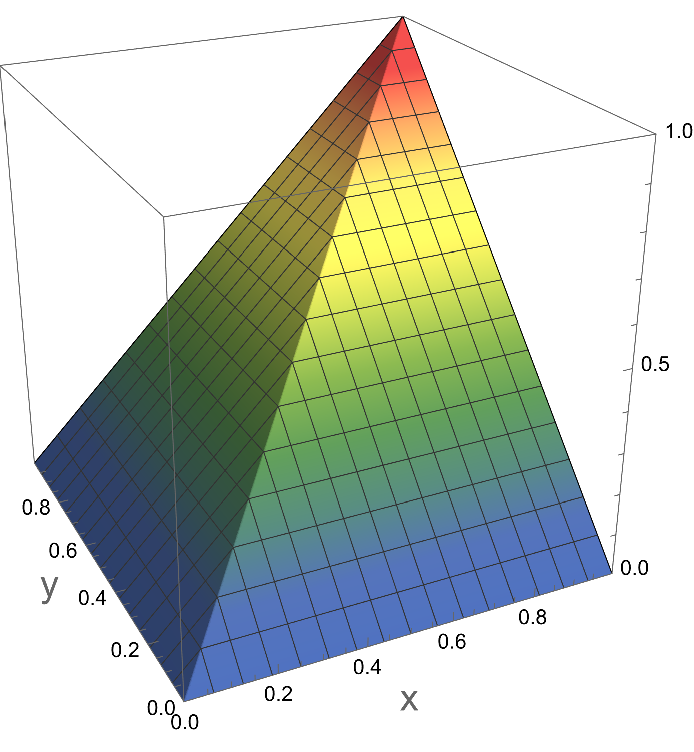
\includegraphics[scale=0.35]{TM.pdf}
		\caption{\TM}
	\end{subfigure}\hspace{0.5cm}
	\begin{subfigure}{.3\textwidth}
		\centering
		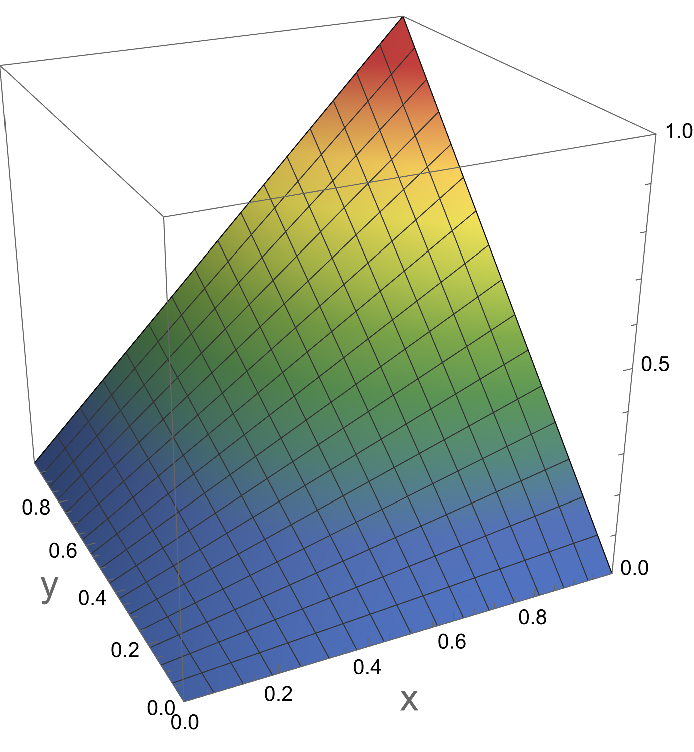
\includegraphics[scale=0.35]{TP.pdf}
		\caption{\TP}
	\end{subfigure}\hspace{0.5cm}
		\begin{subfigure}{.3\textwidth}
		\centering
		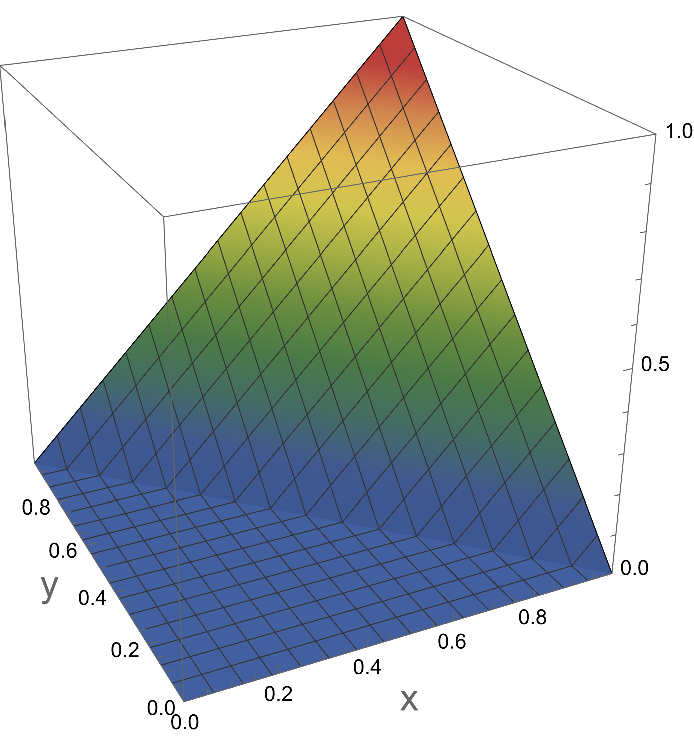
\includegraphics[scale=0.35]{TLK.pdf}
		\caption{\TLK}
	\end{subfigure}\\
	\hspace{0.25cm}
	\begin{subfigure}{.4\textwidth}
		\centering
		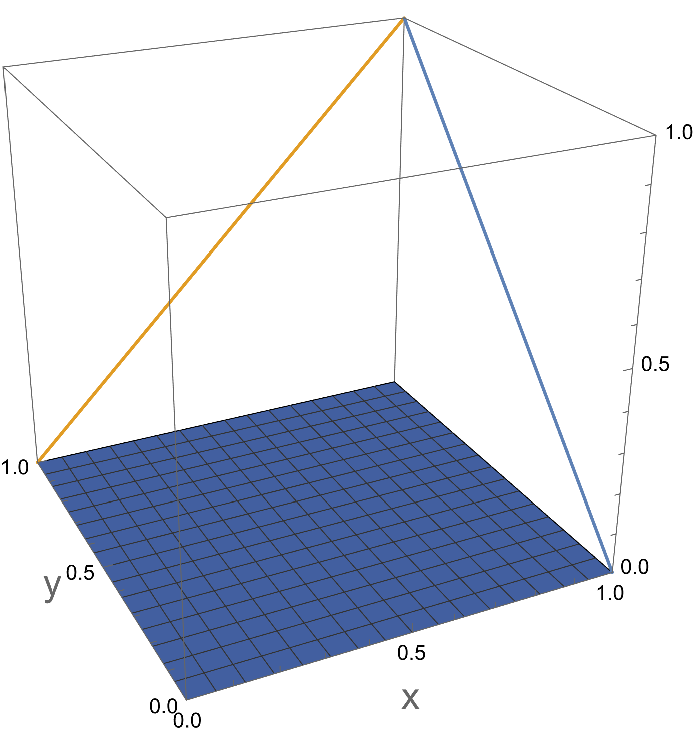
\includegraphics[scale=0.35]{TD.pdf}
		\caption{\TD}
	\end{subfigure}\hspace{0.25cm}
	\begin{subfigure}{.4\textwidth}
	\centering
	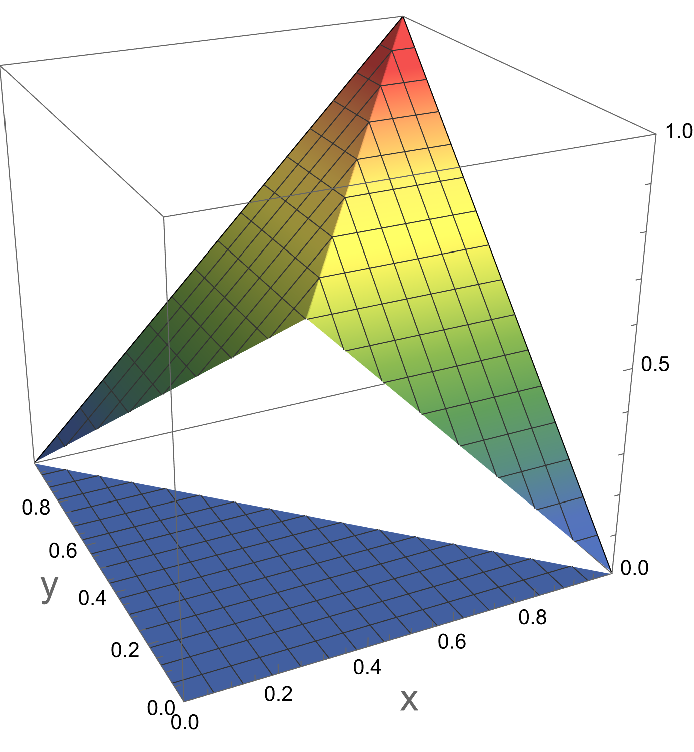
\includegraphics[scale=0.35]{TNM.pdf}
	\caption{$T_{\bm nM}$}
	\end{subfigure}
	\caption{Plots of basic t-norms presented in Table \ref{table:basic_tnorms}.}\label{fig:basic_tnorms}
\end{figure}

\begin{figure}[ht!]
	\centering
	\begin{subfigure}{.3\textwidth}
		\centering
		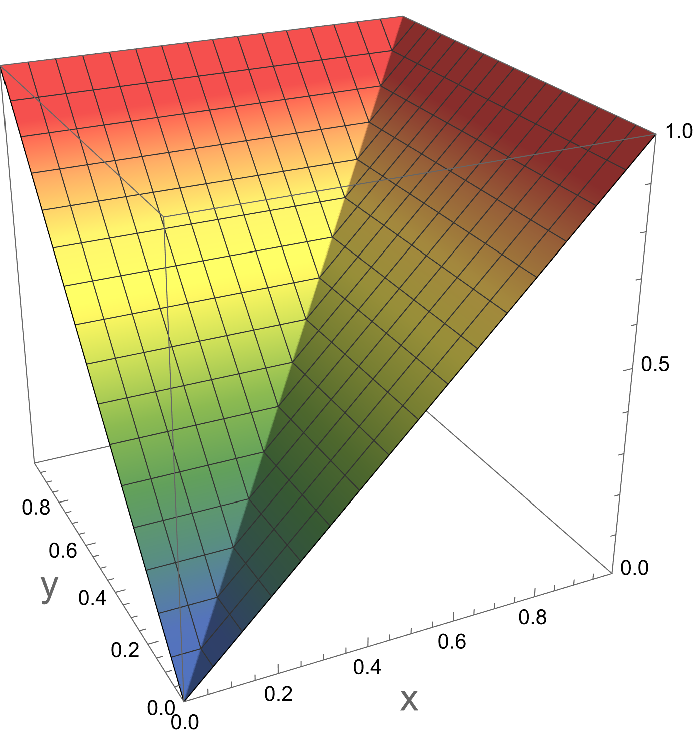
\includegraphics[scale=0.35]{SM.pdf}
		\caption{$S_{\bm M}$}
	\end{subfigure}\hspace{0.5cm}
	\begin{subfigure}{.3\textwidth}
		\centering
		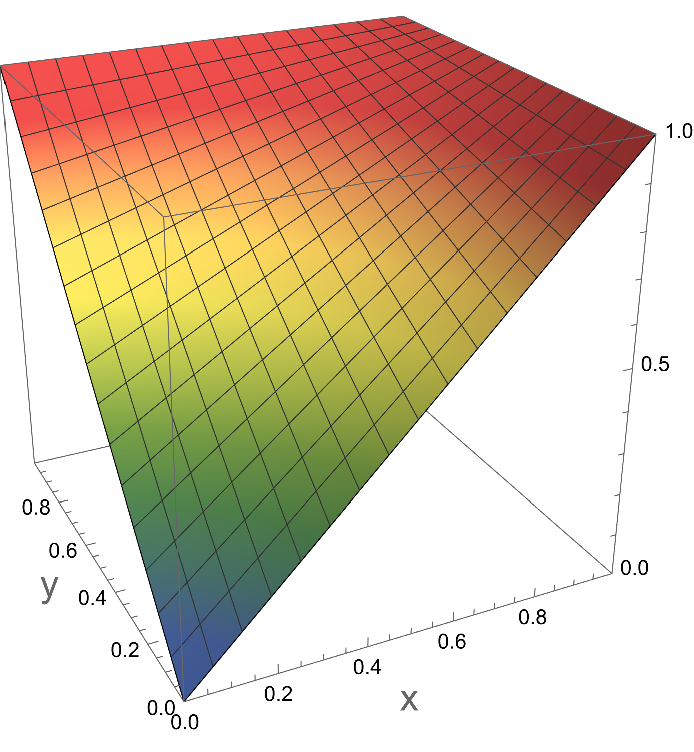
\includegraphics[scale=0.35]{SP.pdf}
		\caption{$S_{\bm P}$}
	\end{subfigure}\hspace{0.5cm}
	\begin{subfigure}{.3\textwidth}
		\centering
		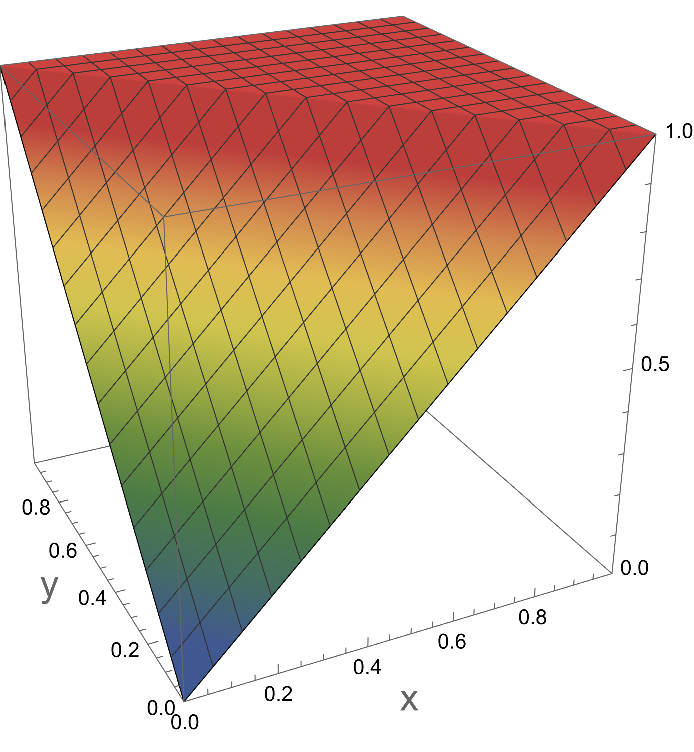
\includegraphics[scale=0.35]{SLK.pdf}
		\caption{$S_{\bm LK}$}
	\end{subfigure}\\
	\hspace{0.25cm}
	\begin{subfigure}{.4\textwidth}
		\centering
		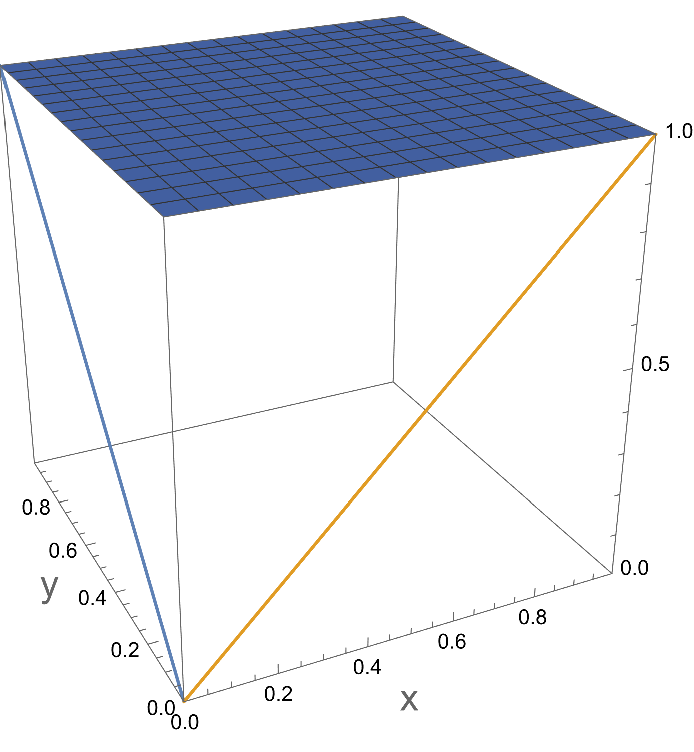
\includegraphics[scale=0.35]{SD.pdf}
		\caption{$S_{\bm D}$}
	\end{subfigure}\hspace{0.25cm}
	\begin{subfigure}{.4\textwidth}
		\centering
		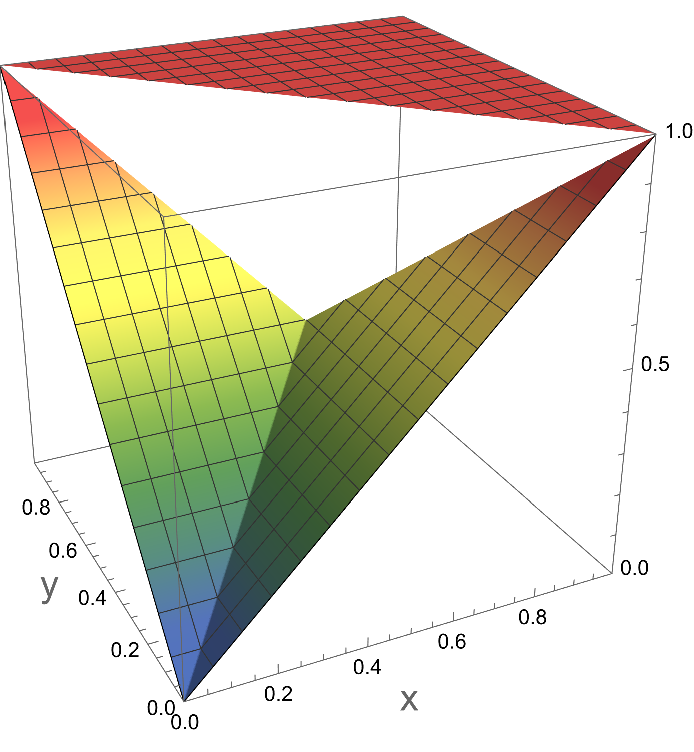
\includegraphics[scale=0.35]{SNM.pdf}
		\caption{$S_{\bm nM}$}
	\end{subfigure}
	\caption{Plots of basic t-conorms presented in Table \ref{table:basic_toconorms}.}\label{fig:basic_tconorms}
\end{figure}

Hereafter, we name several subclasses of t-norms and t-conorms.

\begin{definition}[\bf{\cite[Definition 2.1.2]{Baczynski2008}}] A t-norm $T:[0,1]^2 \to [0,1]$ is called
	\begin{itemize}
		\item \emph{idempotent} if $T(x,x)=x$ for all $x \in [0,1]$;
		\item \emph{positive} if $T(x,y)=0$ implies either $x=0$ or $y=0$;
		\item \emph{cancellative} if $T(x,y)=T(x,z)$ implies $y=z$ for all $x,y,z \in [0,1]$, $x>0$;
		\item \emph{conditionally cancellative} if $T(x,y)=T(x,z)>0$ implies $y=z$ for all $x,y,z \in [0,1]$;
		\item \emph{Archimedean} if for all $x,y \in (0,1)$ there exists an $n \in \NN$ such that $x_T^{(n)}<y$.
	\end{itemize}
\end{definition}

\begin{definition}[\textbf{\cite[Definition 2.13]{Klement2000}}]  A continuous Archimedean t-norm $T:[0,1]^2 \to [0,1]$ is called	
	\begin{itemize}
		\item \emph{strict} if it is strictly increasing on $(0,1]^2$.
		\item \emph{nilpotent} if there exists $(x,y) \in (0,1]^2$ such that $T(x,y)=0$.
	\end{itemize}
	A strict t-norm is cancellative and a nilpotent t-norm is conditionally cancellative.
\end{definition}

\pagebreak

\begin{definition}[\bf{\cite[Definition 2.2.2]{Baczynski2008}}] A t-conorm $S:[0,1]^2 \to [0,1]$ is called
	\begin{itemize}
		\item \emph{idempotent} if $S(x,x)=x$ for all $x \in [0,1]$;
		\item \emph{cancellative} if $S(x,y)=S(x,z)$ implies $y=z$ for all $x,y,z \in [0,1]$, $x<1$;
		\item \emph{conditionally cancellative} if $S(x,y)=S(x,z)<1$ implies $y=z$ for all $x,y,z \in [0,1]$;
		\item \emph{Archimedean} if for all $x,y \in (0,1)$ there exists an $n \in \NN$ such that $x_S^{(n)}>y$.
	\end{itemize}
\end{definition}

\begin{definition}[\textbf{\cite[Remark 2.20]{Klement2000}}]  A continuous Archimedean t-conorm $S:[0,1]^2 \to [0,1]$ is called	
	\begin{itemize}
		\item \emph{strict} if it is strictly increasing on $[0,1)^2$.
		\item \emph{nilpotent} if there exists $(x,y) \in [0,1)^2$ such that $S(x,y)=1$.
	\end{itemize}
	A strict t-conorm is cancellative and a nilpotent t-conorm is conditionally cancellative.
\end{definition}

It is well known that there exists a duality between t-norms and t-conorms which can be expressed in terms of a strictly decreasing bijection $\varphi:[0,1] \to [0,1]$ (see \cite[Proposition 2.34]{Klement2000}). In particular, this duality is usually considered in the case when $\varphi(x)=1-x$ for all $x \in [0,1]$.
\begin{proposition}[\bf{\cite[Proposition 2.2.3]{Baczynski2008}}]\label{prop:duality} For a function $S:[0,1]^2 \to [0,1]$, $S$ is a t-conorm if and only if there exists a t-norm $T:[0,1]^2 \to [0,1]$ such that 
	$$S(x,y)=1-T(1-x,1-y), \quad x,y \in [0,1].$$
	Moreover, the t-norm $T$ is continuous (Archimedean, cancellative, conditionally cancellative) if and only if the t-conorm $S$ is continuous (Archimedean, cancellative, conditionally cancellative).	
\end{proposition}


For instance, each $S_l$ in Figure $\ref{fig:basic_tconorms}$ is dual to $T_l$ in Figure \ref{fig:basic_tnorms} for all $l \in \{M,P,LK,D,nM\}$ in the sense of Proposition \ref{prop:duality}. Thanks to this duality, many results obtained for t-norms can be directly adapted for t-conorms.

Also, given a strong negation $N$ we can define the $N$-dual of a t-norm or a t-conorm, respectively.

\begin{proposition}[\bf{\cite{Klement2000}}]\label{prop:N_dual} Let $N$ be a strong negation, the following statements hold:
	\begin{enumerate}[label=(\roman*)]
		\item For any t-norm $T:[0,1]^2 \to [0,1]$, the function $S: [0,1]^2 \to [0,1]$ defined by
		$$S(x,y)=N(T(N(x),N(y))), \quad x,y \in [0,1],$$
		is a t-conorm called the \emph{$N$-dual of $T$}.
		\item For any t-conorm $S:[0,1]^2 \to [0,1]$, the function $T: [0,1]^2 \to [0,1]$ defined by
		$$T(x,y)=N(S(N(x),N(y))), \quad x,y \in [0,1],$$
		is a t-norm called the \emph{$N$-dual of $S$}.
	\end{enumerate}
\end{proposition}

Consecutively, we give further results of continuous and Archimedean t-norms. Notice that a continuous t-norm is Archimedean if and only if it has only trivial idempotent points, i.e., 0 and 1.

For nilpotent t-norms it is interesting to consider their induced negation, since the points of the t-norm which are equal to zero can be described in terms of this function.

\begin{definition}[\textbf{\cite{Jenei1998}}]
	Let $T$ be a nilpotent t-norm, the \emph{induced negation} of $T$ is defined by
	$$N_T(x) = \max \{t \in [0,1] \mid T(x,t)=0\}, \quad \text{for all } x \in [0,1].$$
\end{definition}

\begin{proposition}[\textbf{\cite{Jenei1998}}]\label{prop:NTinvolutive}
	Let $T$ be a nilpotent t-norm, then $N_T$ is a strong fuzzy negation. Moreover,
	$$T(x,y)=0 \Leftrightarrow N_T(x) \geq y.$$
\end{proposition}

The structure of Archimedean t-norms can be described in terms of a continuous, strictly decreasing function that is unique up to a positive multiplicative constant.

\begin{theorem}[\textbf{\cite[Theorem 5.1]{Klement2000}}]\label{th:representation_archimedeantnorms}
	For a function $T:[0,1]^2 \to [0,1]$ the following statements are equivalent:
	\begin{enumerate}[label=(\roman*)]
		\item $T$ is a continuous Archimedean t-norm.
		\item $T$ has a continuous additive generator, i.e., there exists a continuous, strictly decreasing function $t:[0,1]\to [0,+\infty]$ with $t(1)=0$, which is uniquely determined up to a positive multiplicative constant, such that
		$$ T(x,y)=t^{(-1)}(t(x)+t(y)), \quad \text{for all } x,y \in [0,1],$$
		where $t^{(-1)}$ is the pseudo-inverse of $t$ given by $t^{(-1)}(x)=t^{-1}(\min\{t(0),x\})$ for all $x \in [0,+\infty]$.
	\end{enumerate}
\end{theorem}

Notice that from Theorem \ref{th:representation_archimedeantnorms} we deduce that the difference between a strict and a nilpotent Archimedean t-norm in terms of an additive generator is that the value $t(0)$ is infinite or not, respectively. In addition, the induced negation of a nilpotent t-norm can be expressed in terms of an additive generator.

\begin{remark}\label{remark:gen_negation}
	Let $T$ be a nilpotent t-norm, $N_T$ its induced negation and $t$ an additive generator of $T$. Then,
	$$N_T(x)=t^{-1}(t(0)-t(x)), \quad \text{for all } x \in [0,1].$$
\end{remark}

Moreover, from Theorem \ref{th:representation_archimedeantnorms} it can be derived that there is a duality between additive and multiplicative generators of continuous Archimedean t-norms.

\begin{remark}[\textbf{\cite[Remark 3.34]{Klement2000}}]
	Let $T$ be a continuous Archimedean t-norm and $t: [0,1] \to [0,+\infty]$ an additive generator of $T$. Then $\theta:[0,1] \to [0,1]$ defined by $\theta(x)=e^{-t(x)}$ for all $x \in [0,1]$ is a multiplicative generator of $T$, i.e., it is a strictly increasing function with $\theta(1)=1$ such that
	$$T(x,y)=\theta^{(-1)}(\theta(x)\cdot\theta(y)), \quad \text{for all } x,y \in [0,1].$$
\end{remark}

\begin{example}[\textbf{\cite{Klement2000}}]\label{ex:Lukasiewicz} The most well-known continuous Archimedean t-norms are the product t-norm \TP and the Łukasiewicz t-norm \TLK (see Table \ref{table:basic_tnorms} and Figure \ref{fig:basic_tnorms}). In fact, continuous Archimedean t-norms can be represented as the $\Phi$-conjugates of these two t-norms \cite[Propositions 5.9 and 5.10]{Klement2000}. The additive generators of \TP and \TLK are
$$t(x)=-k\ln(x), \quad t(x)=k(1-x),$$
for all $x \in [0,1]$ and $k>0$, respectively. Moreover, the induced negation of \TLK is $N_{\TLK}(x)=1-x$ for all $x \in [0,1]$.
\end{example}

Now, we recall the following proposition that contains two results about nilpotent t-norms that involve the induced negation and disclose some information about their structure. Since we have obtained these results from more general results of left-continuous t-norms we provide the explicit proof.

\begin{proposition}[\textbf{\cite{Jenei1998}}]
	\label{prop:PropertiesNT}
	Let $T$ be a nilpotent t-norm and $N_T$ its induced negation. The following statements hold:
	\begin{enumerate}[label=(\roman*)]
		\item Let $x \in (0,1]$ and $h_x : [N_T(x),1] \to [0,x]$ be the function defined by $h_x(y)=T(y,x)$. Then $h_x$ is continuous, strictly increasing and
		$$h_x^{-1}(z)=N_T(T(N_T(z),x)), \quad \text{for all } z \in [0,x].$$
		\item Let $x_1,x_2,y_1,y_2 \in [0,1]$. If $T(x_1,y_1)=T(x_2,y_2)>0$, then 
		$$T(N_T(x_1),y_2)=T(N_T(x_2),y_1).$$
	\end{enumerate}
\end{proposition}

\begin{proof}
	\begin{enumerate}[label=(\roman*)]
		\item Since a nilpotent t-norm is conditionally cancellative and due to Proposition \ref{prop:NTinvolutive} it is straightforward that $h_x$ is continuous and strictly increasing. Since $T$ is nilpotent, it is continuous and, in particular, is left-continuous and $N_T$ is a strong negation. Then by \cite[(i)-Theorem 2]{Jenei1998} for all $x \in (0,1]$ and $z \in[0,x]$ we have
		\begin{eqnarray*}
		N_T(T(x,N_T(z))) &=& \sup \{ t \in [0,1] \mid T(x,t) \leq z\} = \max \{t \in [0,1] \mid t \leq h_x^{-1}(z)\} \\
		&=& h_x^{-1}(z).
		\end{eqnarray*}
		\item Since $T(x_1,y_1), T(x_2,y_2)>0$ by Proposition \ref{prop:NTinvolutive} we have $N_T(x_1)<y_1$ and $N_T(x_2)<y_2$. Then by the fact that $N_T$ is involutive and by (i) we have
		$$h_{y_1}^{-1}(N_T(x_1))=N_T(T(x_1,y_1))=N_T(T(x_2,y_2))=h_{y_2}^{-1}(N_T(x_2)),$$
		and then
		\begin{eqnarray*}
			T(N_T(x_1),y_2) & = & T(T(h_{y_1}^{-1}(N_T(x_1)),y_1),y_2) = T(T(h_{y_1}^{-1}(N_T(x_1)),y_2),y_1) \\
			& = & T(T(h_{y_2}^{-1}(N_T(x_2)),y_2),y_1) = T(N_T(x_2),y_1).
		\end{eqnarray*}
	\end{enumerate}
\end{proof}

Another fact that reflects the importance of continuous Archimedean t-norms relies on the characterization of continuous t-norms, which states that a continuous t-norm can be described in terms of an ordinal sum of continuous Archimedean t-norms.

\begin{theorem}[\textbf{\cite[Theorem 5.11]{Klement2000}}]\label{th:characcontt-norm}
	For a function $T:[0,1]^2 \to [0,1]$ the following statements are equivalent:
	\begin{enumerate}[label=(\roman*)]
		\item $T$ is a continuous t-norm.
		\item $T$ is uniquely representable as an ordinal sum of continuous Archimedean t-norms, i.e., there exist a uniquely determined (finite or countably infinite) index set $A$, a family of uniquely determined pairwise disjoint open sub-intervals $\{(a_{\alpha},e_{\alpha})\}_{\alpha \in A}$ of $[0,1]$ and a family of uniquely determined continuous Archimedean t-norms $(T_{\alpha})_{\alpha \in A}$ such that
		$$T(x,y)
		=
		\left\{\begin{array}{ll}
			a_{\alpha}+(e_{\alpha}-a_{\alpha})\cdot T_{\alpha}\left(\frac{x-a_{\alpha}}{e_{\alpha}-a_{\alpha}},\frac{y-a_{\alpha}}{e_{\alpha}-a_{\alpha}}\right) & \text{if } x,y \in [a_{\alpha},e_{\alpha}), \\
			\min\{x,y\} & \text{otherwise.}
		\end{array}
		\right.
		$$
		In this case, we will write $T=(\langle a_{\alpha},e_{\alpha},T_{\alpha}\rangle)_{\alpha \in A}$.
	\end{enumerate}
\end{theorem}

% Powers of a t-norm
The powers of a t-norm $T$ generalize the notion of the diagonal (2nd power of a t-norm). In {\cite{Walker2002}} the $r$-th powers with respect to continuous t-norms are studied in detail, so we only include here  a brief description. From the associativity of any t-norm $T$, positive integer powers with respect to $T$ can be defined in the usual way (see Equation \ref{eq:powers:genF}), that is,
$$x_T^{(n)} = \overbrace{T(x,T(x,\dots,T(x,x)))}^{n \ times} = T(\overbrace{x,x,\ldots,x}^{n \ times}) \quad \text{for all} \  x\in[0,1], \ n\in \NN \text{ and } n\geq 2,$$
with the conventions $x_T^{(1)}=x$ and  $x_T^{(0)}=1$ for all $x \in [0,1]$.

Similarly, $n$-th roots and positive rational powers of an element $x \in [0,1]$ with respect to a t-norm $T$ are defined as
\[
x_T^{\left(\frac{1}{n}\right)}=\sup\{z \in [0,1] \ | \ z_T^{(n)}\leq x\}, \qquad  x_T^{\left(\frac{m}{n}\right)}=\left(x_T^{\left(\frac{1}{n}\right)}\right)_T^{(m)},
\]
for all $m,n \in \NN$.

\begin{lemma}[\bf{\cite{Walker2002}}]
	\label{fraccions equivalents}
	Consider $k,m,n \in \NN$ and let  $T$ be a continuous t-norm. Then $x_T^{\left(\frac{km}{kn}\right)}=x_T^{\left(\frac{m}{n}\right)}$ for all $x\in[0,1]$.
\end{lemma}

From the continuity of $T$, positive rational powers with respect to $T$ can be extended to positive irrational powers through the following definition. 

\begin{definition}[\bf{\cite{Walker2002}}]
	\label{potencies irracionals}
	Let $T$ be a continuous t-norm and $r$ a positive real number. Consider $\{a_n \}_{n\in \NN}$ a sequence of rational numbers such that $\displaystyle \lim_{n \to +\infty}a_n=r$. For all $x \in [0,1]$, the power $x_T^{(r)}$ is defined as
	\[
	x_T^{(r)}=\displaystyle \lim_{n \to +\infty}x_T^{(a_n)}.
	\]
	We can extend the definition to $r=+\infty$ in the same way and then
	\[
	x_T^{(+\infty)}=\displaystyle \lim_{n \to +\infty}x_T^{(a_n)},
	\]
	where $\{a_n \}_{n\in \NN}$ is a sequence of positive rational numbers such that $\displaystyle \lim_{n \to +\infty}a_n=+\infty$.
\end{definition} 

The continuity of $T$ ensures both, the existence of the limit and the independence of the considered sequence $\{a_n \}_{n\in \NN}$. It is immediate to check that $0\leq x_T^{(r)}\leq 1$ and $x_T^{(r)}\leq y_T^{(r)}$ whenever $x\leq y$ for all $x,y\in[0,1]$ and  $r\in [0,+\infty]$. 

When the selected t-norm is Archimedean, the $r$-th powers can be expressed in terms of an additive generator.

\begin{proposition}[\bf{\cite{Walker2002}}]
Let $T$ be a continuous Archimedean t-norm with additive generator $t$. Then,
$$x_T^{(r)}=t^{-1}(\min\{t(0),rt(x)\}), \quad \text{for all } x \in [0,1] \text{ and } r \in [0,+\infty],$$
with the convention that $+\infty \cdot 0 = 0$.
\end{proposition}


\subsection{Uninorms}
Uninorms are associative functions that were defined as a generalization of t-norms and t-conorms \cite{Yager1996} by allowing any element $e \in [0,1]$ to act as a neutral element.

\begin{definition}[\bf{\cite{Yager1996,Klement2000}}]\label{def:uninorm}
	A binary operator $U:[0,1]^2 \to [0,1]$ is said to be a \emph{uninorm} if there exists $e \in [0,1]$, called \emph{neutral element}, such that $U$ satisfies:
	\begin{description}
		\item[(U1)] $U(x,y)=U(y,x)$ for all $x,y \in [0,1]$. \hfill (Commutativity)
		\item[(U2)] $U(x,U(y,z))=U(U(x,y),z)$ for all $x,y,z \in [0,1]$. \hfill (Associativity)
		\item[(U3)] $U(x,y) \leq U(x,z)$ when $y \leq z$, for all $x,y,z \in [0,1]$. \hfill (Monotonicity)
		\item[(U4)] $U(x,e)=x$ for all $x \in [0,1]$. \hfill (Neutral element)
	\end{description}
\end{definition}

From Definition \ref{def:uninorm} it is clear that $U$ is a t-norm if $e=1$ and a t-conorm if $e=0$. Thus, in order to distinguish these operators from these particular cases we say that a uninorm is \emph{proper} if $e \in (0,1)$. Besides, it holds that $U(1,0) \in \{0,1\}$ and we say that $U$ is \emph{conjunctive} if $U(1,0)=0$ and \emph{disjunctive} if $U(1,0)=1$.

The structure of uninorms is more complex than t-norms and t-conorms, so usually these operators are classified in different families \cite{Mas2015}. Some well-known characterized families of uninorms can be found hereunder.

\subsubsection{Uninorms in $\mathcal{U}_{\min}$ and $\mathcal{U}_{\max}$}

\begin{theorem}[\textbf{\cite[Theorem 1]{Mas2015}}]
	Let $U$ be a uninorm with neutral element $e \in (0,1)$.
	\begin{enumerate}[label=(\roman*)]
		\item If $U(0,1)=0$ and the function $U(\cdot,1)$ is continuous except in $x=e$, then $U$ is given by
		\begin{equation}\label{eq:umin}
			U(x,y)
			=
			\left\{\begin{array}{ll}
				e \cdot T_U\left(\frac{x}{e},\frac{y}{e}\right) & \text{if } x,y \in [0,e], \\
				e + (1-e) \cdot S_U\left(\frac{x-e}{1-e},\frac{y-e}{1-e}\right) & \text{if } x,y \in [e,1], \\
				\min\{x,y\} & \text{otherwise.}
			\end{array}
			\right.
		\end{equation}
		\item If $U(0,1)=1$ and the function $U(\cdot,0)$ is continuous except in $x=e$, then $U$ is given by
		\begin{equation}\label{eq:umax}
			U(x,y)
			=
			\left\{\begin{array}{ll}
				e \cdot T_U\left(\frac{x}{e},\frac{y}{e}\right) & \text{if } x,y \in [0,e], \\
				e + (1-e) \cdot S_U\left(\frac{x-e}{1-e},\frac{y-e}{1-e}\right) & \text{if } x,y \in [e,1], \\
				\max\{x,y\} & \text{otherwise.}
			\end{array}
			\right.
		\end{equation}
	\end{enumerate}
	In both formulas $T_U$ is a t-norm and $S_U$ is a t-conorm. The class of uninorms of the form (\ref{eq:umin}) is denoted by $\mathcal{U}_{\min}$, while the class of uninorms of the form (\ref{eq:umax}) is denoted by $\mathcal{U}_{\max}$.
\end{theorem}

\subsubsection{Idempotent uninorms}

\begin{definition}[\textbf{\cite[Definition 5.1.5]{Baczynski2008}}]
	A uninorm $U$ such that $U(x,x)=x$ for all $x \in [0,1]$ is said to be an \emph{idempotent uninorm}. The class of all idempotent uninorms is denoted by $\mathcal{U}_{Idem}$.
\end{definition}

\begin{theorem}[\textbf{\cite[Theorem 5]{Mas2015}}]
	For a function $U : [0,1]^2 \to [0,1]$ the following statements are equivalent:
	\begin{enumerate}[label=(\roman*)]
		\item $U$ is an idempotent uninorm with neutral element $e \in [0,1]$.
		\item There exists a decreasing function $g: [0,1] \to [0,1]$, symmetric with respect to the main diagonal, with $g(e)=e$, such that
		\begin{equation}\label{eq:uidempotent}
			U(x,y)
			=
			\left\{\begin{array}{ll}
				\min\{x,y\} & \text{if } y<g(x) \text{ or } (y=g(x) \text{ and } x<g(g(x))), \\
				\max\{x,y\} & \text{if } y>g(x) \text{ or } (y=g(x) \text{ and } x>g(g(x))), \\
				x \text{ or } y & \text{if } y=g(x) \text{ and } x=g(g(x)), \\
			\end{array}
			\right.
		\end{equation}
	being commutative in the points $(x,y)$ such that $y=g(x)$ with $x=g(g(x))$.
	\end{enumerate}
\end{theorem}

%\begin{center}
%	\textsc{Representable Uninorms}
%\end{center}

\subsubsection{Representable uninorms}

\begin{definition}[\textbf{\cite[Theorem 5.1.12]{Baczynski2008}}]
	A uninorm $U$ is called \emph{representable} if it has a continuous additive generator, i.e., there exists a continuous and strictly increasing function $h:[0,1] \to [-\infty,+\infty]$ such that $h(0)=-\infty$, $h(e)=0$ for an $e \in (0,1)$ and $h(1)=+\infty$, which is uniquely determined up to a positive multiplicative constant, such that
	$$U(x,y)
	=
	\left\{\begin{array}{ll}
		0 & \text{if } (x,y) \in \{(0,1),(1,0)\}, \\
		h^{-1}(h(x)+h(y)) & \text{otherwise},
	\end{array}
	\right.
	$$
	or 
	$$U(x,y)
	=
	\left\{\begin{array}{ll}
		1 & \text{if } (x,y) \in \{(0,1),(1,0)\}, \\
		h^{-1}(h(x)+h(y)) & \text{otherwise}.
	\end{array}
	\right.
	$$
	The class of all representable uninorms is denoted by  $\mathcal{U}_{Rep}$.
\end{definition}

For more details regarding uninorms we refer the reader to \cite{Mas2015} and references therein.

\subsection{Copulas}

Copulas are binary operators $C:[0,1]^2 \to [0,1]$ that were originated in the context of statistics and play a major role in Sklar's theorem, which states that any two-dimensional distribution function can be written in terms of two marginal distribution functions and a copula, which describes the dependence between the variables \cite{Sklar1959,Nelsen1999}. However, copulas are also studied as fuzzy conjunctions which, unlike t-norms, are not necessarily commutative or associative.
\begin{definition}[\textbf{\cite[Definition 2.2.2]{Nelsen1999}}]
	A \emph{copula} is a function $C: [0,1]^2 \to [0,1]$ which satisfies the following conditions:
	\begin{enumerate}[label=(\roman*)]
		\item $C(x,0)=C(0,y)=0$ for all $x,y \in [0,1]$.
		\item $C(x,1)=x$ for all $x \in [0,1]$.
		\item $C(1,y)=y$ for all $y \in [0,1]$.
		\item Let, $x_1,x_2,y_1,y_2 \in [0,1]$ such that $x_1 \leq x_2$ and $y_1 \leq y_2$, then
		$$C(x_2,y_2)-C(x_2,y_1)-C(x_1,y_2)+C(x_1,y_1) \geq 0.$$
	\end{enumerate}
\end{definition}

\begin{example}
There exist many different families of copulas but, according to \cite{Sriboonchitta2018} the Farlie-Gumbel-Morgenstern (FGM) copula is one of the most important:
$$C(x,y)=x \cdot y + \theta \cdot x \cdot (1-x) \cdot y \cdot (1-y),$$
for all $x,y \in [0,1]$ and $\theta \in [-1,1]$.
\end{example}

For more details regarding copulas and other related operators we refer the reader to \cite{Nelsen1999,Beliakov2010,Calvo2002,Grabisch2009}.


\section{Fuzzy implication functions}\label{section:fuzzy_implication_functions}

Similarly to fuzzy negations, t-norms or t-conorms, fuzzy implication functions are a generalization of the corresponding classical operator to fuzzy logic. In this section we give the definition of a fuzzy implication function, we recall some of their main additional properties and we provide several examples. Also, we present the families that are related to the results of this monograph.

\subsection{Definition and additional properties}\label{subsection:definition&additionalproperties}
The most accepted definition of fuzzy implication functions is the following one.
\begin{definition}[\bf{\cite{Baczynski2008,Fodor1994}}]\label{defimp}
	A binary operator $I:[0,1]^2 \to [0,1]$ is said to be a \emph{fuzzy implication function} if it satisfies:
	\begin{description}
		\item[\Ione]  $I(x,z)\geq I(y,z)\ $  when  $\ x\leq y$, for all $x,y,z\in[0,1]$. \hfill (Left Antitonicity)
		\item[\Itwo]  $I(x,y)\leq I(x,z)\ $  when  $\ y\leq z$, for all $x,y,z\in[0,1]$. \hfill (Right Isotonicity)
		\item[\Ithree]  $I(0,0)=I(1,1)=1$ and $I(1,0)=0$. \hfill (Boundary Condition)
	\end{description}
\end{definition}
If we recall the truth table of the classical implication
\begin{center}
	\begin{tabular}{|c|c|c|}
		\hline
		$p$ & $q$ & $p \to q$ \\ \hline
		0   & 0   & 1         \\ \hline
		0   & 1   & 1         \\ \hline
		1   & 0   & 0         \\ \hline
		1   & 1   & 1         \\ \hline
	\end{tabular}
\end{center}
\noindent it is clear that the boundary condition \Ithree ensures that a fuzzy implication function restricted to $\{0,1\}^2$ coincides with the classical implication (note that $I(0,1)=1$ is guaranteed due to $I(0,0)=1$ and \Itwo. In addition, \Ione incorporates the idea that a lower truth value of the first variable is more efficient to state more about the truth value of its consequent. On the other hand, \Itwo is connected to the idea that the overall truth value depends on the consequent directly.

From Definition \ref{defimp} it can be easily derived that $I(0,x) = I(x,1) = 1$ for all $x \in [0, 1]$. However, the values $I(x,0)$ and $I(1,x)$ are not predetermined by the definition. In fact, the values $I(x,0)$ define what is called the natural negation of a fuzzy implication function.
\begin{definition}[\textbf{\cite[Definition 1.4.14]{Baczynski2008}}]\label{def:naturalnegationI}
	Let $I$ be a fuzzy implication function. The function $N_I:[0,1] \to [0,1]$ defined by
	$$N_I(x)=I(x,0), \quad \text{for all } x \in [0,1],$$
	is a fuzzy negation called the \emph{natural negation} of $I$.
\end{definition}

\begin{remark}
	For the sake of simplicity, some results related to the characterization of fuzzy implication functions use the notation $N_I$ where $I:[0,1]^2 \to [0,1]$ is an arbitrary binary function. When $I$ is not a fuzzy implication function this notation refers to the horizontal section $I(\cdot,0)$, which may not be a fuzzy negation.
\end{remark}

Since Definition \ref{defimp} is quite general, additional properties of these operators are usually considered. These properties come often in the form of functional equations which involve fuzzy implication functions and some of them, other operators as well. The motivation behind the definition of these additional properties are diverse, but the most usual are: a large majority of them were introduced as the straightforward generalizations of classical logic tautologies to fuzzy logic; others point out some desirable or interesting analytical/algebraic properties of these functions; some were introduced since they appeared when solving a particular problem; finally, many of these properties aim to be useful in a particular problem or application. Since a lot of additional properties have been introduced in the literature, we limit ourselves to list here the most popular and the ones that are relevant to the results presented in this monograph.

\begin{itemize}
	\item The \emph{left neutrality principle}
	$$I(1,y)=y, \quad y\in[0,1]. \eqno {\text{\NP}}$$
	\item The \emph{exchange principle} 
	$$I(x,I(y,z)) = I(y,I(x,z)), \quad  x,y,z\in[0,1]. \eqno {\text{\EP}}$$
	\item The \emph{identity principle} 
	$$ I(x,x)=1, \quad x\in[0,1]. \eqno {\text{\IP}}$$
	\item The \emph{ordering property} 
	$$I(x,y)=1 \Leftrightarrow x \leq y, \quad x,y\in[0,1]. \eqno {\text{\OP}}$$
	\item The \emph{consequent boundary}
	$$ I(x,y)\geq y, \quad x,y \in [0,1]. \eqno {\text{\CB}}$$
	\item The \emph{iterative boolean law}
	$$ I(x,y)=I(x,I(x,y)), \quad x,y \in [0,1]. \eqno {\text{\IB}}$$
	\item The \emph{lowest falsity property}
	$$ I(x,y)=0 \Leftrightarrow x=1 \text{ and } y=0. \eqno {\text{\LF}}$$
	\item The \emph{lowest truth property}
	$$ I(x,y)=1 \Leftrightarrow x=0 \text{ or } y=1. \eqno {\text{\LT}}$$
	\item The \emph{contrapositive symmetry} with respect to a fuzzy negation $N$
	$$ I(x,y)=I(N(y),N(x)), \quad x,y \in [0,1]. \eqno {\text{\CPN}}$$
	\item The \emph{law of left contraposition} with respect to a fuzzy negation $N$
	$$ I(N(x),y)=I(N(y),x), \quad x,y \in [0,1]. \eqno {\text{\LCP}}$$
	\item The \emph{law of right contraposition} with respect to a fuzzy negation $N$
	$$ I(x,N(y))=I(y,N(x)), \quad x,y \in [0,1]. \eqno {\text{\RCPN}}$$
	\item The \emph{law of importation} with respect to a t-norm $T$ 
	$$I(T(x,y),z) = I(x,I(y,z)), \quad  x,y,z\in[0,1]. \eqno {\text{\LI}}$$
	\item The \emph{left neutrality principle with $e\in (0,1) $}
	$$I(e,y)=y, \quad y\in[0,1]. \eqno {\text{\NPe}}$$
	\item  The \emph{$T$-conditionality} with respect to a t-norm $T$
	$$ T(x,I(x,y)) \leq y, \quad x,y \in [0,1]. \eqno {\text{\TC}}$$
	\item The \emph{distributivity laws} with respect to a t-norm $T$ and a t-conorm $S$
	$$I(S(x,y),z)=T(I(x,z),I(y,z)), \quad x,y,z \in [0,1]. \eqno {\text{\DST}}$$
	$$I(T(x,y),z)=S(I(x,z),I(y,z)), \quad x,y,z \in [0,1]. \eqno {\text{\DTS}}$$
	$$I(x,T(y,z))=T(I(x,y),I(x,z)), \quad x,y,z \in [0,1]. \eqno {\text{\DTT}}$$
	$$I(x,S(y,z))=S(I(x,y),I(x,z)), \quad x,y,z \in [0,1]. \eqno {\text{\DSS}}$$
		\item The \emph{$T$-power invariance} with respect to a continuous t-norm $T$
	$$I(x,y)=I\left(x_T^{(r)}, y_T^{(r)}\right), \eqno {\text{\PIT}}$$
	for all positive real numbers $r > 0$ and $x, y \in (0,1)$ such that $x_T^{(r)}, y_T^{(r)} \not = 0$.
\end{itemize}

\begin{remark}\label{remark:PITmodification}
	The definition of the $T$-power invariance with respect to a continuous t-norm $T$ considered in this thesis presents a slight modification with respect to the original one introduced in \cite{Massanet2017}. Specifically, the original definition (see \cite[Definition~5]{Massanet2017}) considers the equality \PIT on the points $x,y \in [0,1]$ such that $x_T^{(r)}, y_T^{(r)} \not = 0,1$, so it also takes into account the $T$-powers of zero. When assuming the original definition, one must take into account that when a non-strict t-norm $T$ is considered, it may happen that $0_T^{(r)}>0$ for some $r>0$. For instance if $T=\TLK$ then $0_{\TLK}^{0.5}=0.5$. Nonetheless, in \cite{Massanet2017} and subsequent papers \cite{Massanet2019,Massanet2019B} the authors rule out the plausible case $x_T^{(r)} \not = 0$ or $y_T^{(r)} \not = 0$ with $x=0$ or $y=0$ in some proofs (see for instance \cite[Propositions 11 and 12]{Massanet2019B}). In view of this situation, we have chosen to modify the corresponding definition to suit the way in which the authors have interpreted it in the results, i.e., discarding the evaluation of the equation $I(x,y)=I\left(x_T^{(r)}, y_T^{(r)}\right)$ when $x$, $y$, $x_T^{(r)}$ or $y_T^{(r)}$ are 0 or 1. This assumption results in the modified definition we have introduced above.  In this interpretation, the boundaries of the unit square are avoided on the two sides of the equation, and not only on the right side. It is clear that the two interpretations may lead to different results, but the comparison of the two perspectives has been considered beyond the scope of this thesis. Thus, throughout the report we consider the modified definition which is also the one used in the results in the existing literature \cite{Massanet2017,Massanet2019,Massanet2019B}.
\end{remark}

Many of these properties, which are not guaranteed by Definition \ref{defimp}, play a major role for a particular application. For instance:
\begin{itemize}
	\item The $T$-conditionality is required in approximate reasoning when the generalized modus ponens as inference mechanism is considered \cite{Baczynski2008}.
	\item  The law of importation \LI and the distributivity laws are useful for reducing the complexity of fuzzy inference mechanisms that involve fuzzy implication functions \cite{Combs1998,Jayaram2008,Jayaram2008B}. Besides, \LI is also considered for the definition of a fuzzy mathematical morphology with good algebraic properties \cite{Kerre2000}.
	\item The lowest falsity and lowest truth properties are needed for the construction of strong equality indices \cite{Bustince2013}.
	\item The ordering property \OP and the law of contraposition \CPN have been useful for constructing some measures from fuzzy implication functions employed in image processing \cite{Bustince2007,Bustince2008}.
	\item The invariance property \PIT, which is thoroughly studied in Chapter \ref{chapter:tpowerinvariant}, is derived from a potential demand in approximate reasoning when fuzzy implication functions are used to model fuzzy conditionals that involve linguistic modifiers \cite{Massanet2017}.
\end{itemize}

Apart from potential applications, the research on additional properties is of the utmost importance in the study of classes of fuzzy implication functions. Indeed, these properties aim to give a proper classification of fuzzy implication functions and to disclose the intersection between different classes. For instance, in Section \ref{subsection:families} the characterization of several families of fuzzy implication functions is recalled, and from these results, we can clearly see how some of these properties are the key of the characterization of the structure of the corresponding class. On the other hand, the study of additional properties can be generally considered as the study of different functional equations. The interrelationships between some of these properties are studied in \cite{Shi2010}.

In Table \ref{table:basic_implications} examples of fuzzy implication functions can be found. Moreover, in Figure \ref{fig:basic_implications} there is the plot of these examples.

\begin{table}[ht!]
	\centering
	\begin{tabular}{|C{3cm}|l|} \hline
		\bf Name & \multicolumn{1}{|c|}{\bf Formula} \\   
		\hline \bf {\L}ukasiewicz & $\ILK(x,y)=\min\{1,1-x+y\}$ \\
		\hline \bf Gödel & $\IGD(x,y)=\left\{\begin{array}{ll}1&\hbox{if } x\leq y\\y&\hbox{if } x>y\end{array}\right.$ \\
		\hline \bf Reichenbach & $\IRC(x,y)=1-x+xy$  \\
		\hline \bf Kleene-Dienes & $\IKD(x,y)=\max\{1-x,y\}$ \\
		\hline \bf Goguen & $\IGG(x,y)=\left \{\begin{array}{ll} 1& \hbox{if } x\leq y\\ \frac{y}{x}&\hbox{if } x>y\end{array}\right.$ \\
		\hline \bf Rescher & $\IRS(x,y)=\left \{\begin{array}{ll} 1& \hbox{if } x\leq y\\ 0&\hbox{if } x>y\end{array}\right.$ \\
		\hline \bf Yager & $\IYG(x,y)=\left \{\begin{array}{ll} 1& \hbox{if } x=0 \hbox{ and } y=0\\ y^x&\hbox{if } x>0 \hbox{ or } y>0\end{array}\right.$ \\
		\hline \bf Weber & $\IWB(x,y)=\left \{\begin{array}{ll} 1& \hbox{if } x<1\\ y&\hbox{if } x=1\end{array}\right.$  \\
		\hline \bf Fodor & $\IFD(x,y)=\left \{\begin{array}{ll} 1& \hbox{if } x\leq y\\ \max\{1-x,y\}&\hbox{if } x>y\end{array}\right.$  \\
		\hline \bf Least & $\ILT(x,y)=\left\{\begin{array}{ll} 1&\hbox{if } x=0 \hbox{ or } y=1\\ 0&\hbox{if } x>0 \hbox{ and } y<1 \end{array}\right.$ \\
		\hline \bf Greatest & $\IGT(x,y)=\left\{\begin{array}{ll} 1&\hbox{if } x<1 \hbox{ or } y>0\\ 0&\hbox{if } x=1 \hbox{ and } y=0 \end{array}\right.$ \\
		\hline
	\end{tabular}
	\caption{Basic Fuzzy Implication Functions.}\label{table:basic_implications}
\end{table}

\begin{figure}[htp!]
	\centering
	\subfloat[\ILK]{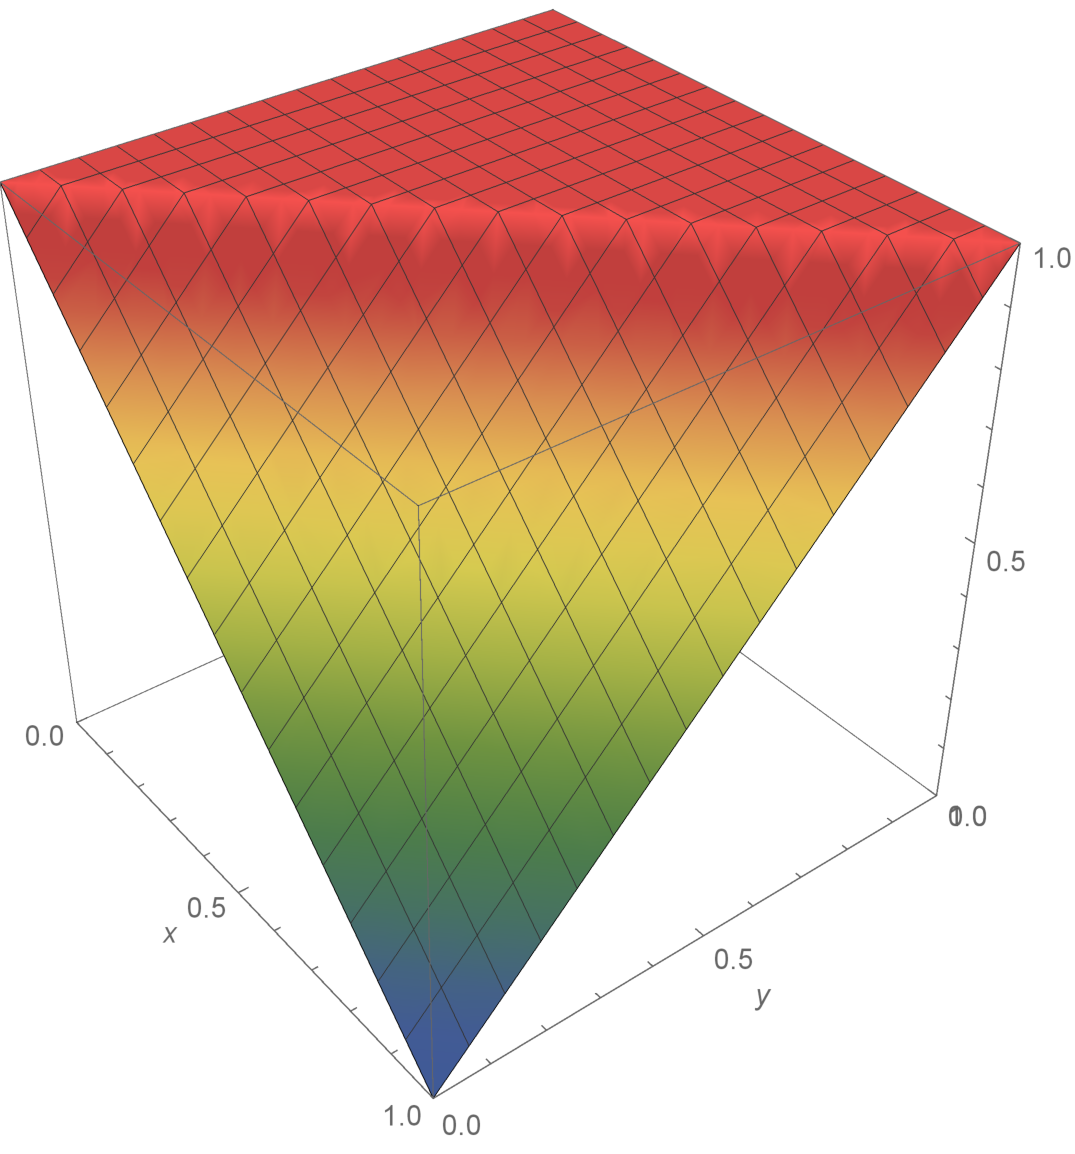
\includegraphics[width=4cm]{ILK.pdf} }
	\subfloat[\IGD]{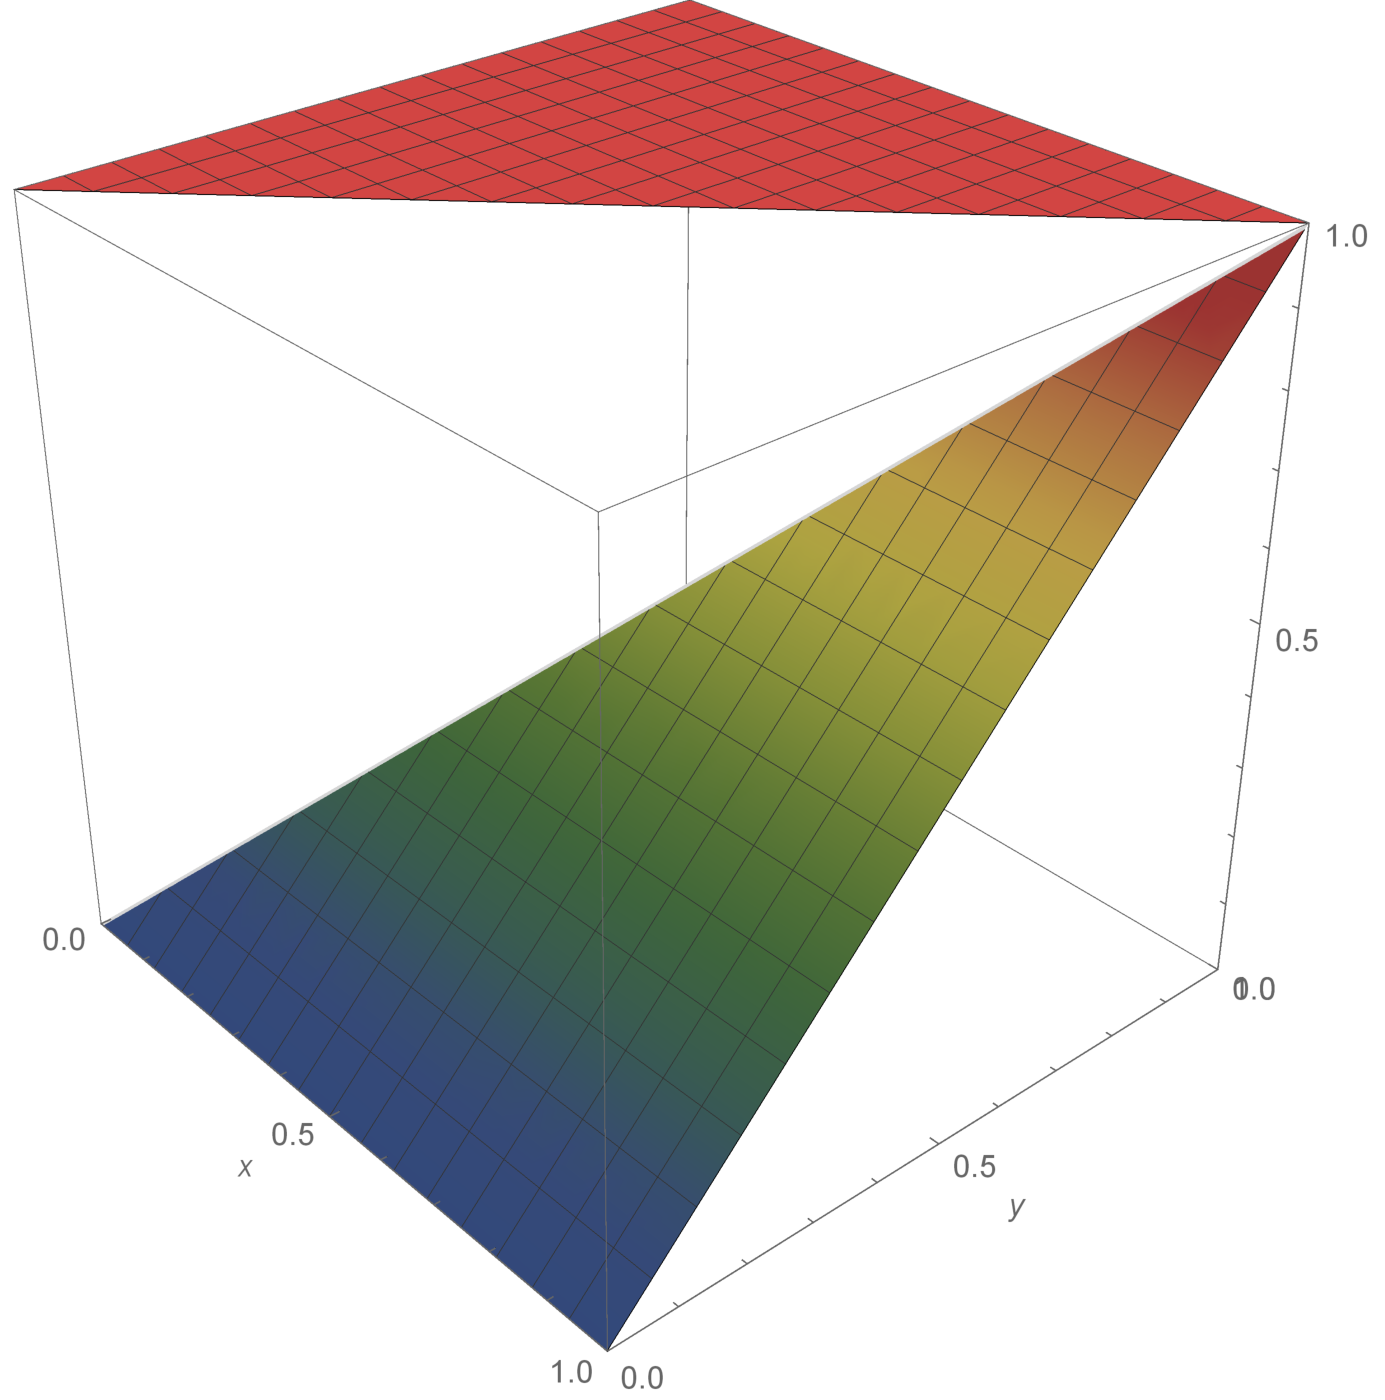
\includegraphics[width=4cm]{IGD.pdf} }
	\subfloat[\IRC]{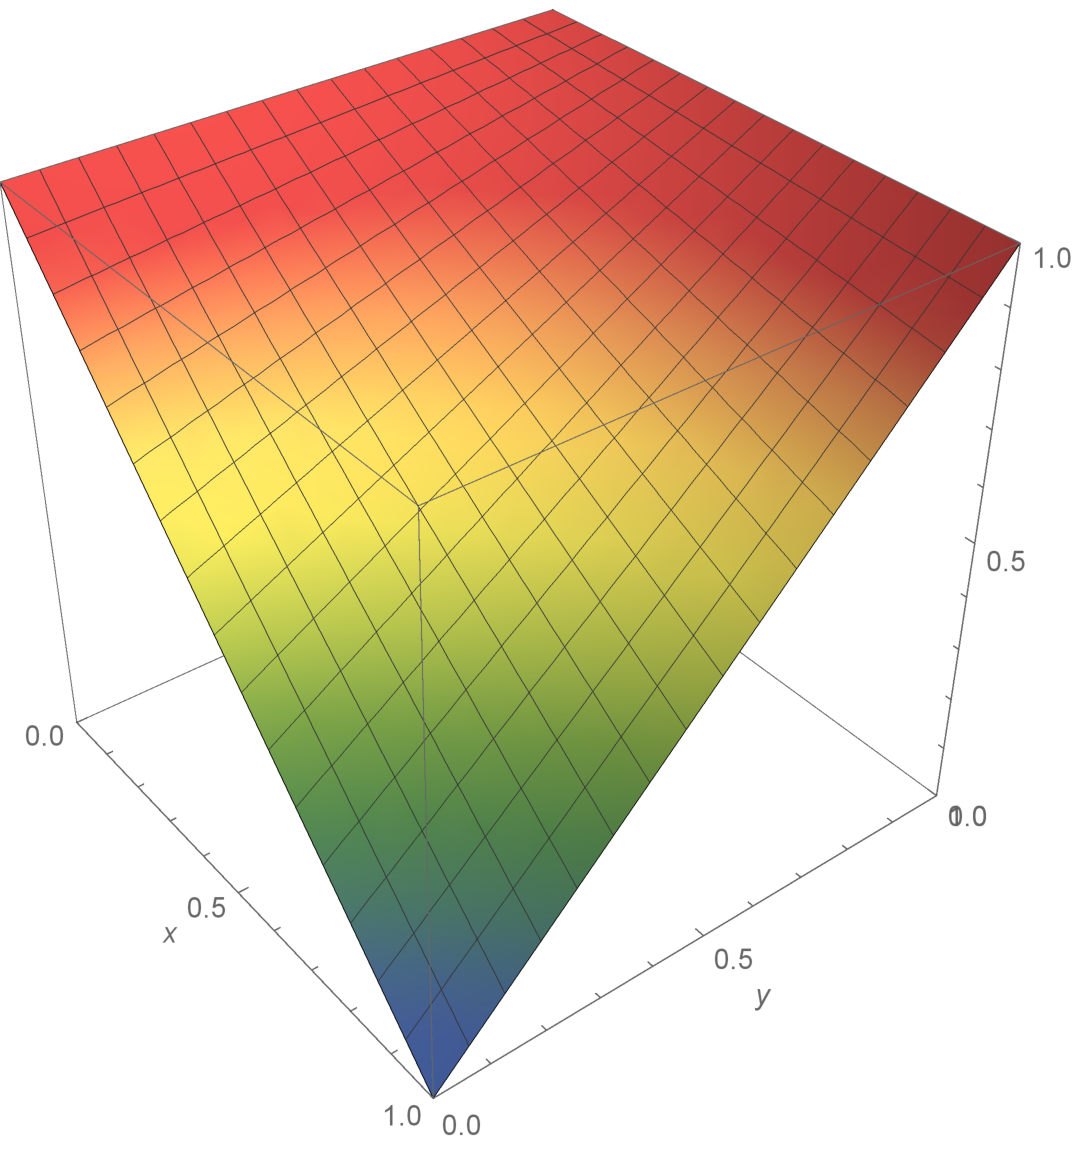
\includegraphics[width=4cm]{IRC.pdf} }\\
	\subfloat[\IKD]{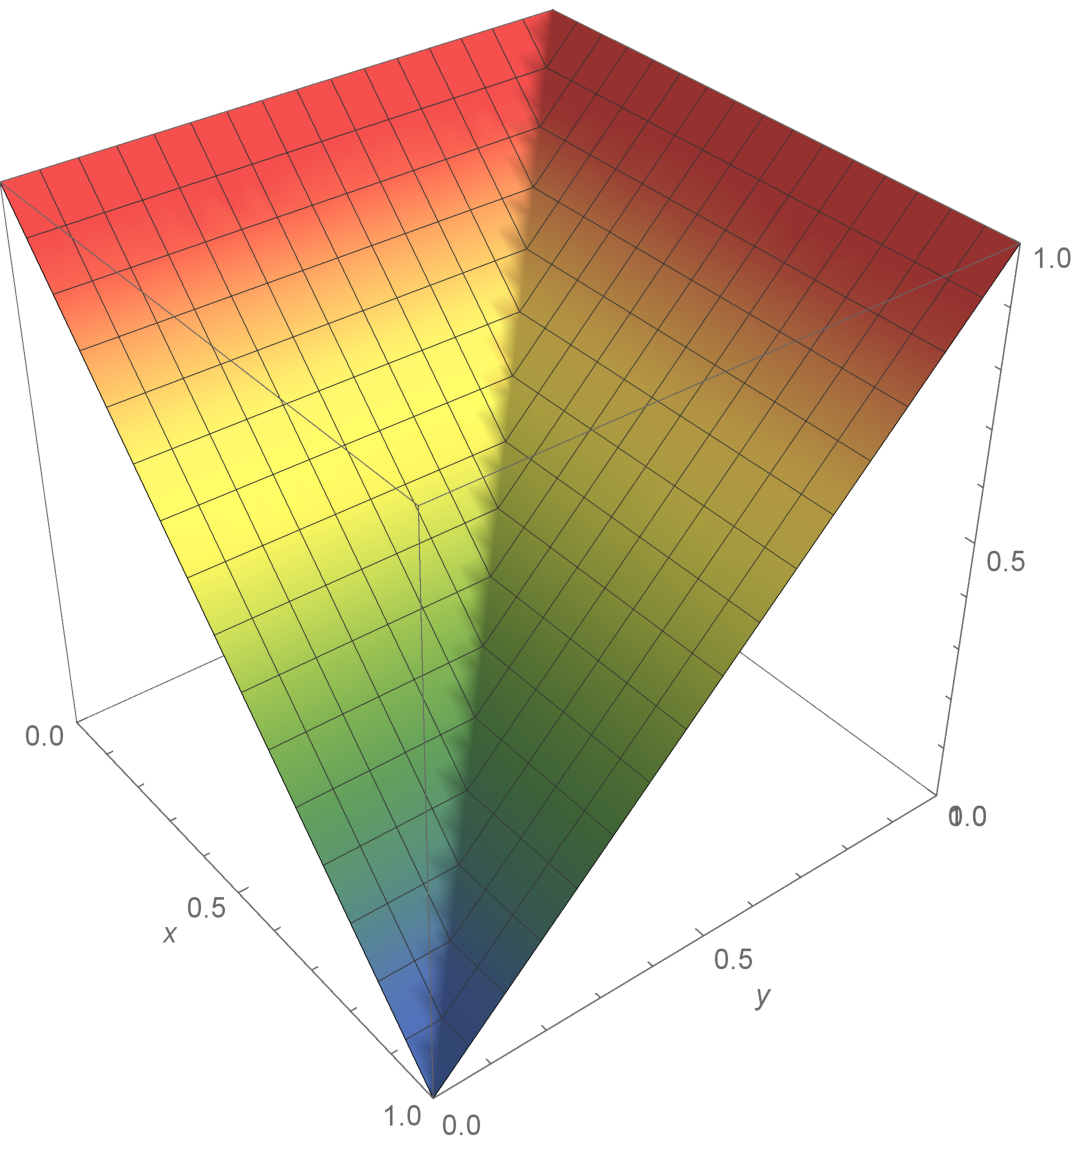
\includegraphics[width=4cm]{IKD.pdf} }
	\subfloat[\IGG]{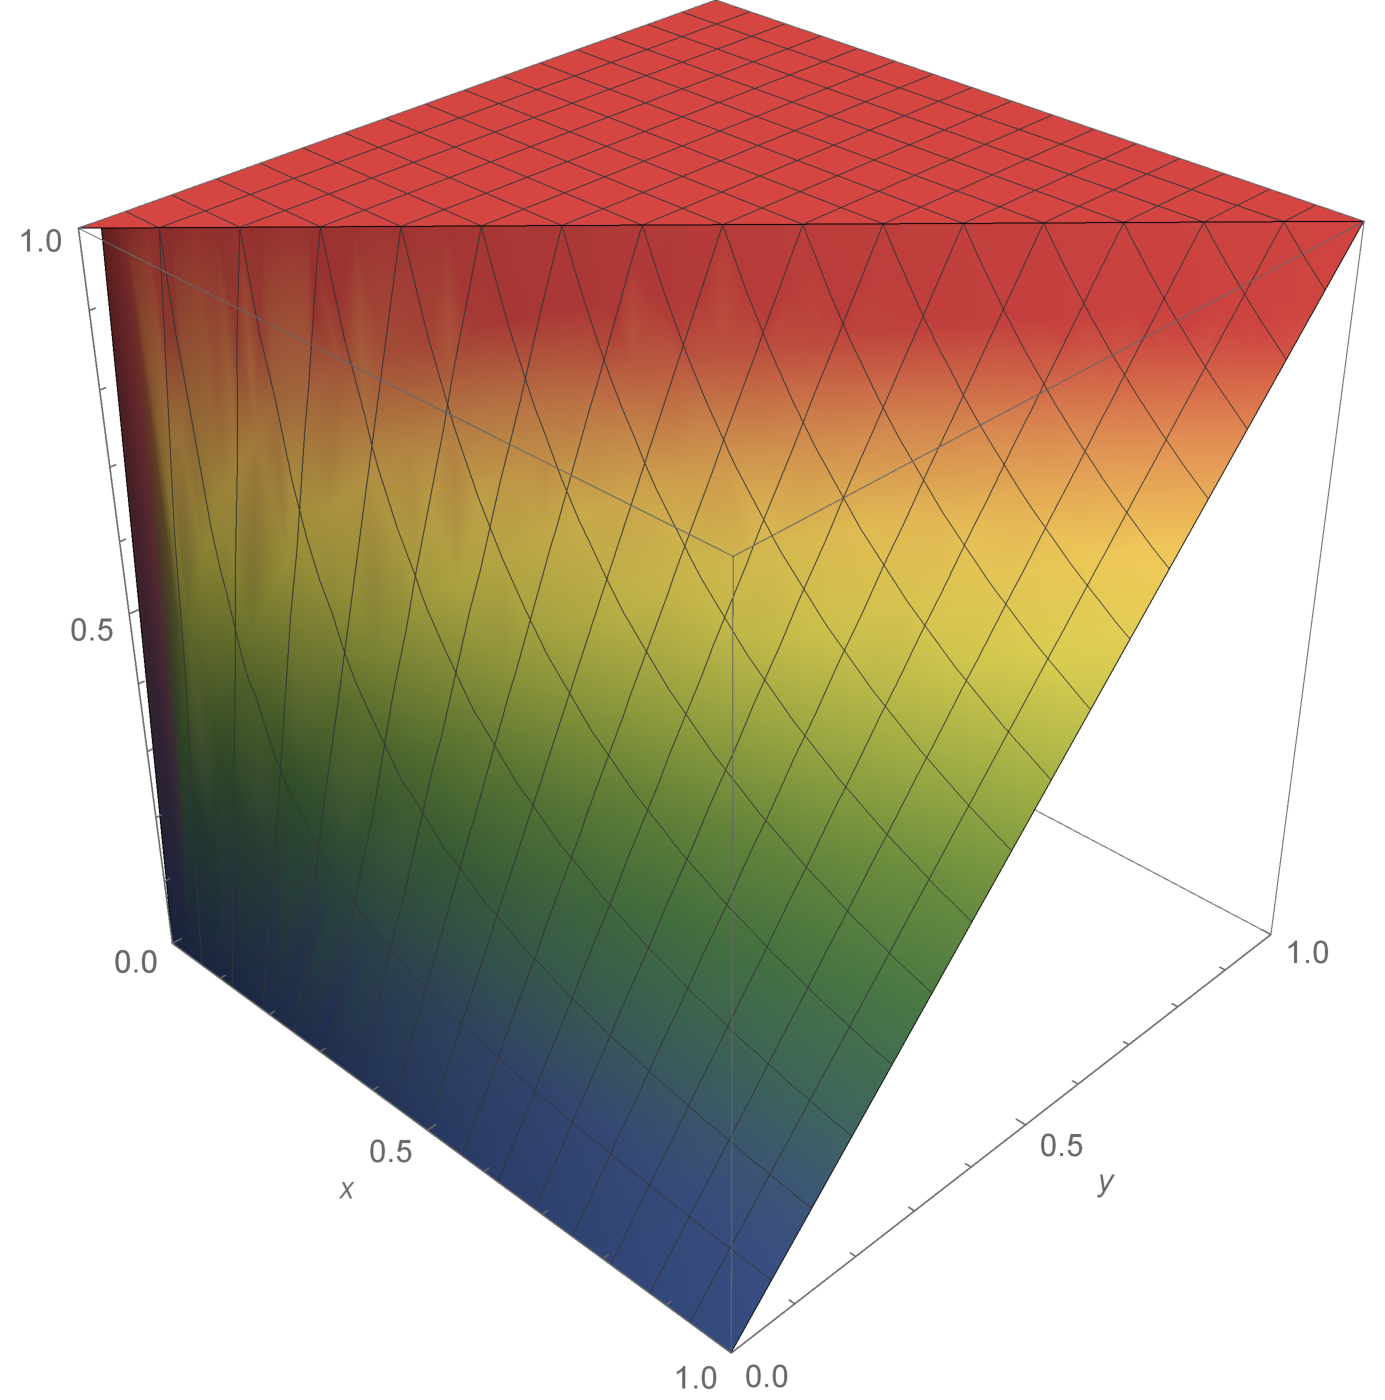
\includegraphics[width=4cm]{IGG.pdf} }
	\subfloat[\IRS]{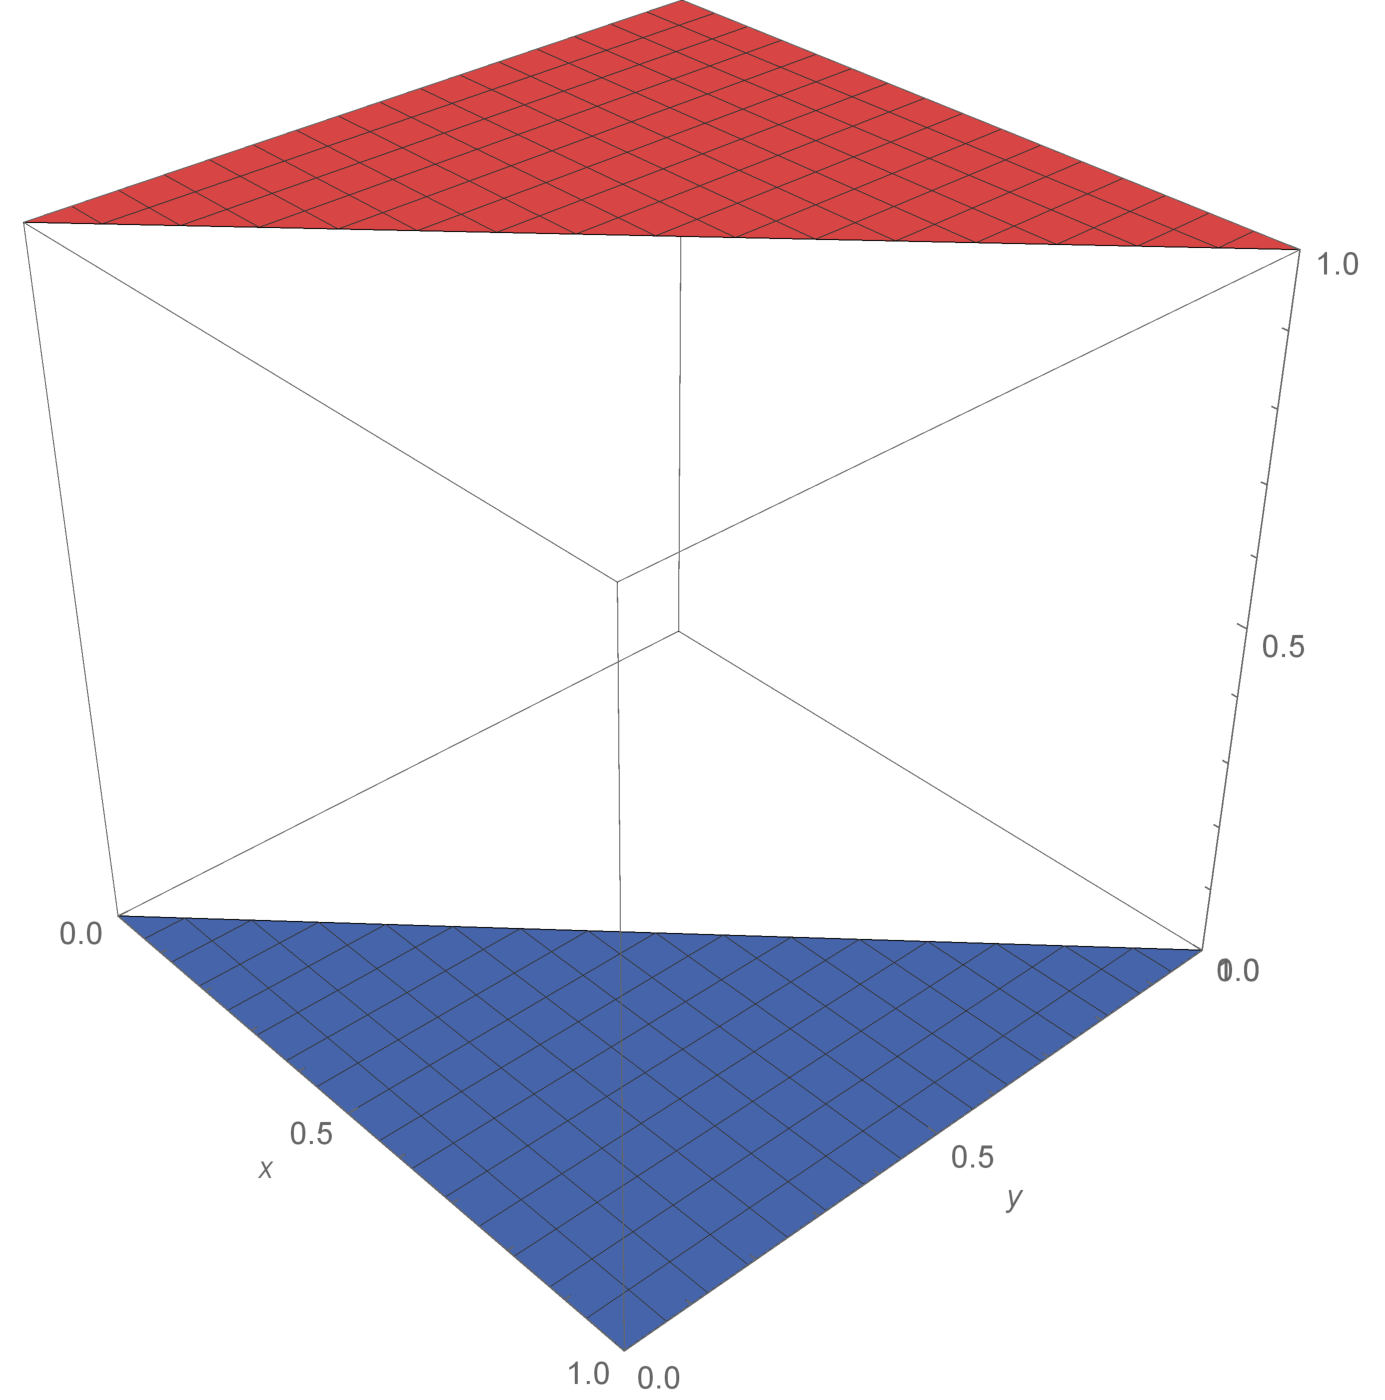
\includegraphics[width=4cm]{IRS.pdf} }\\
	\subfloat[\IYG]{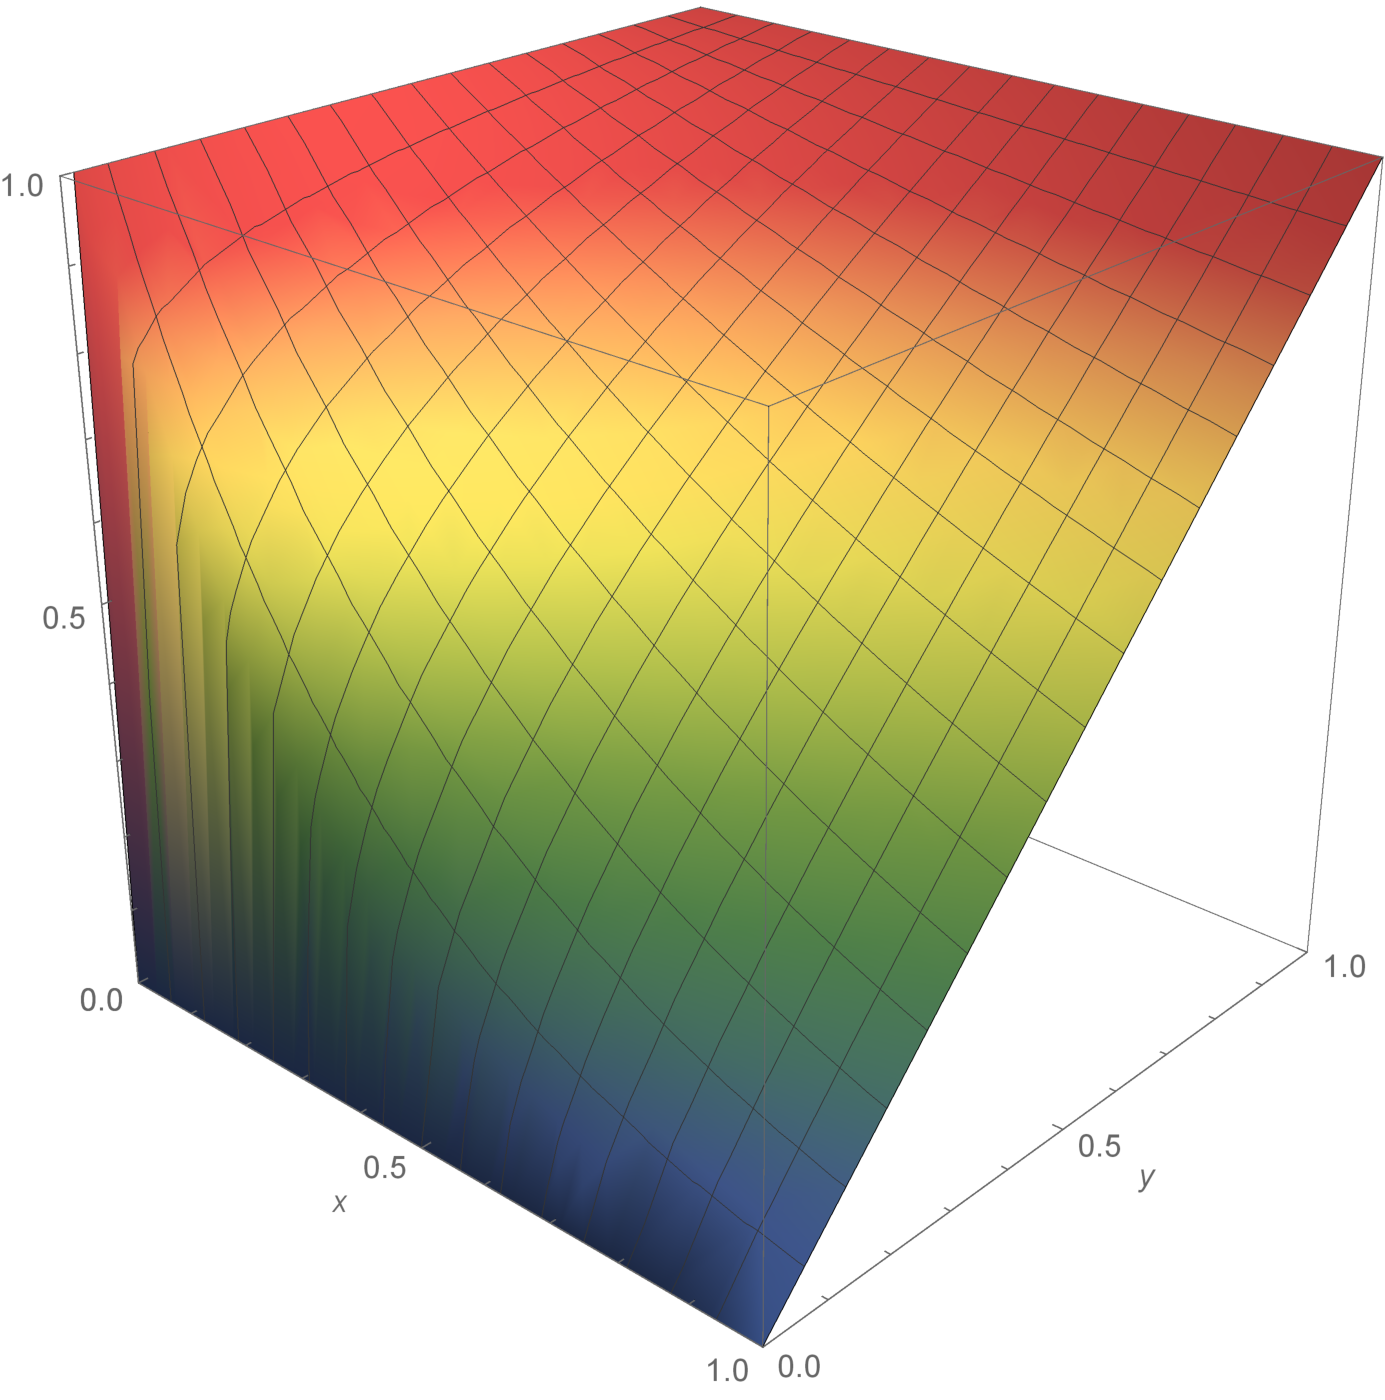
\includegraphics[width=4cm]{IYG.pdf} }
	\subfloat[\IWB]{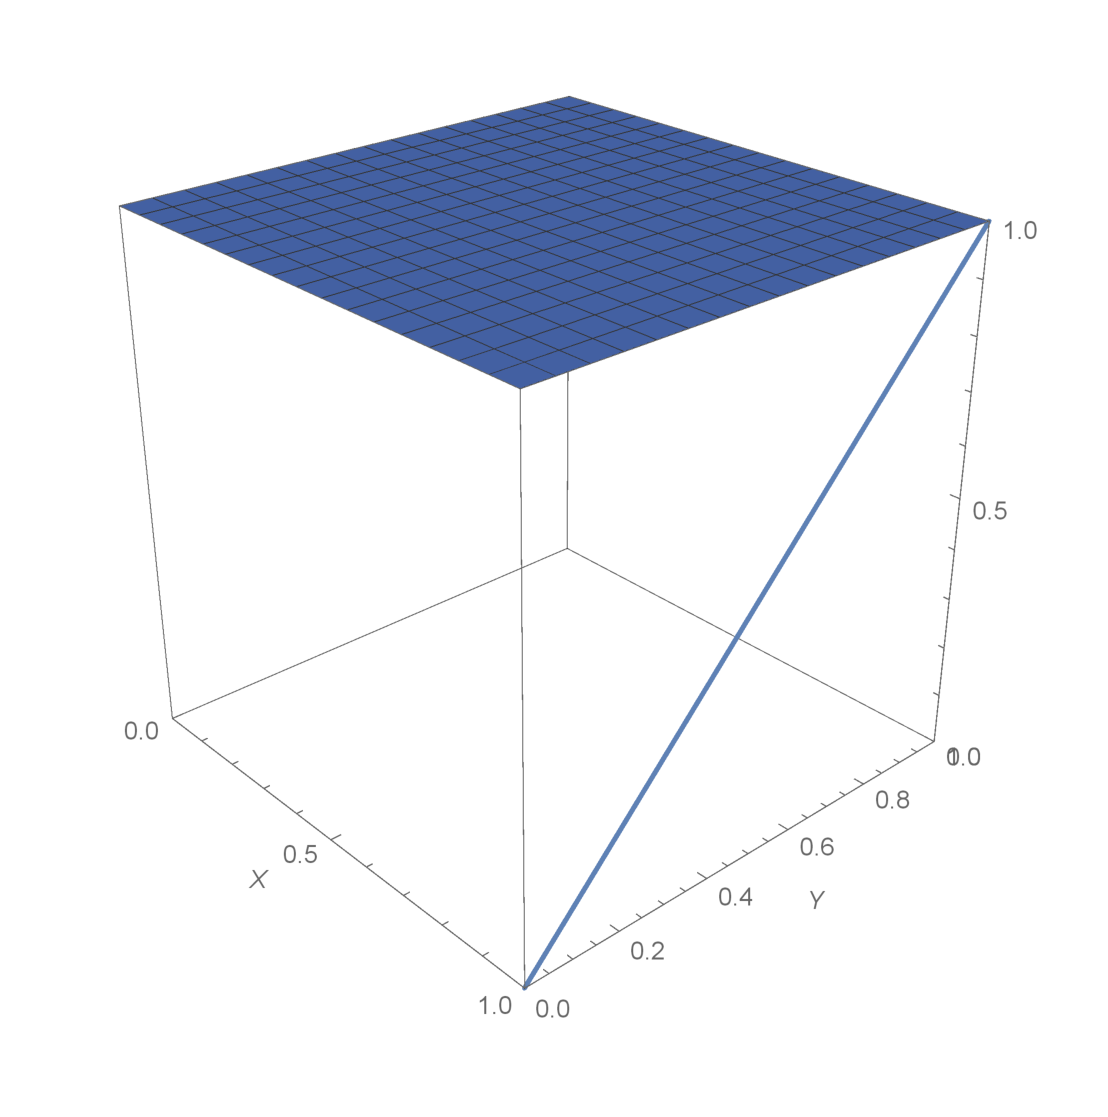
\includegraphics[width=4.5cm]{IWB.pdf} }
	\subfloat[\IFD]{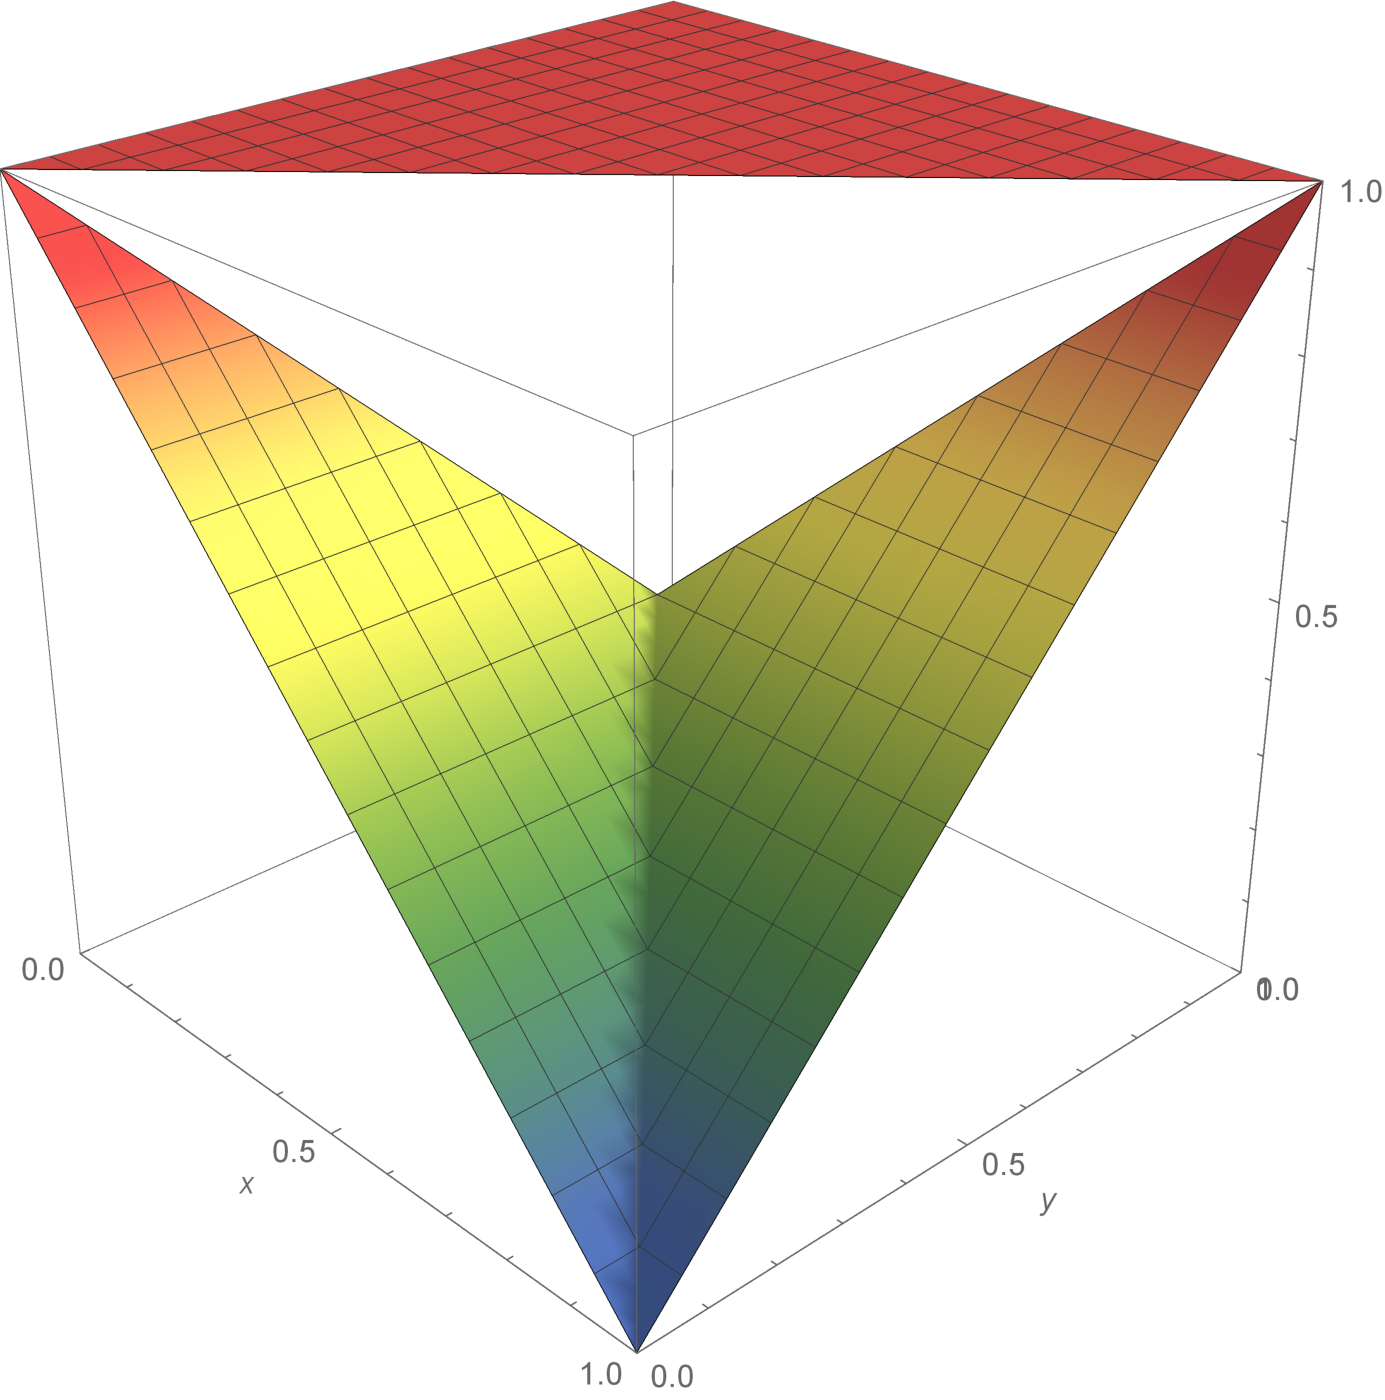
\includegraphics[width=4cm]{IFD.pdf} }\\
	\subfloat[\ILT]{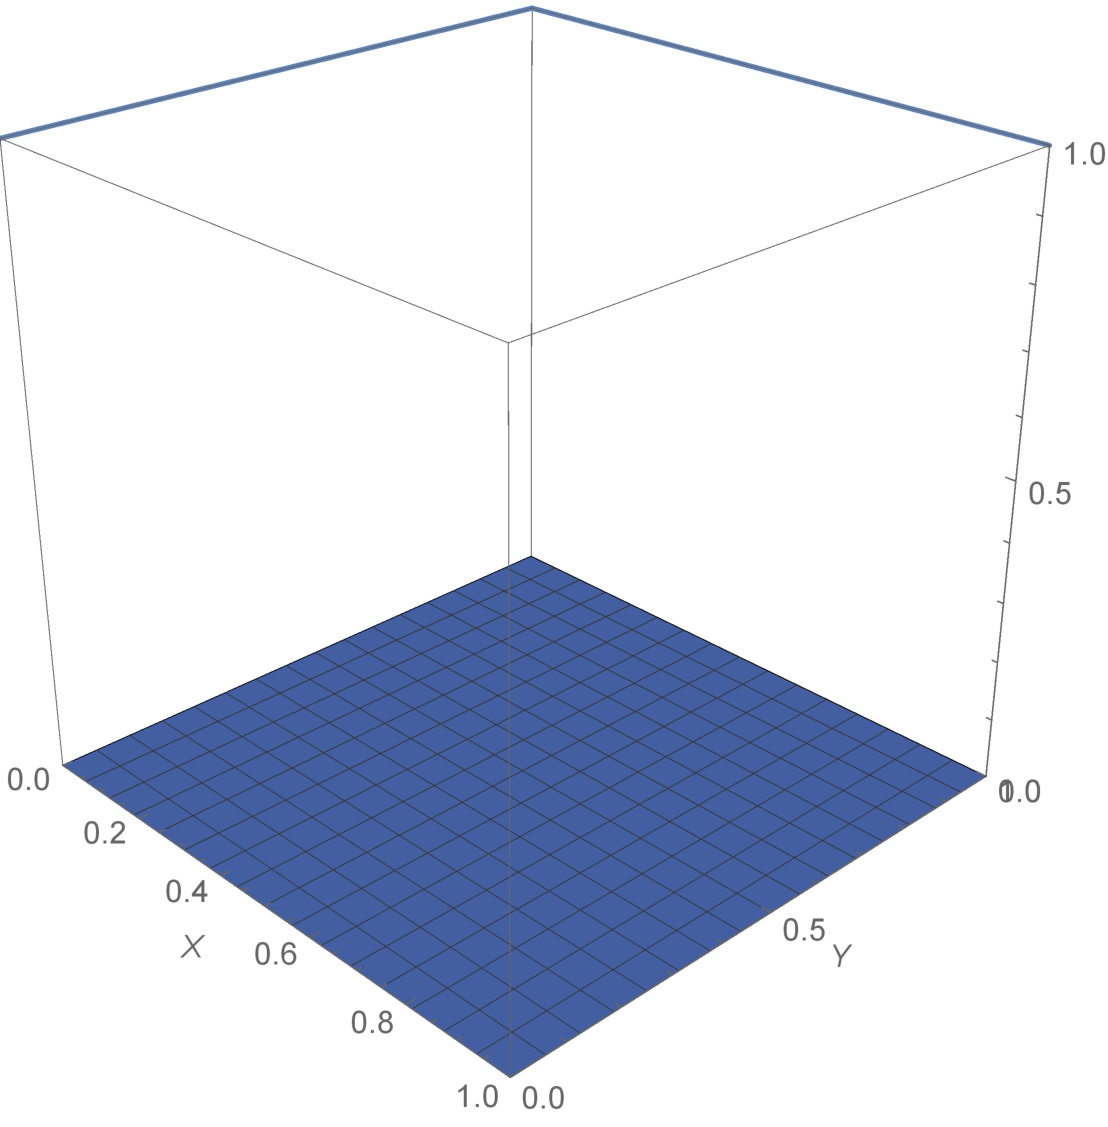
\includegraphics[width=4cm]{ILT.pdf} }
	\subfloat[\IGT]{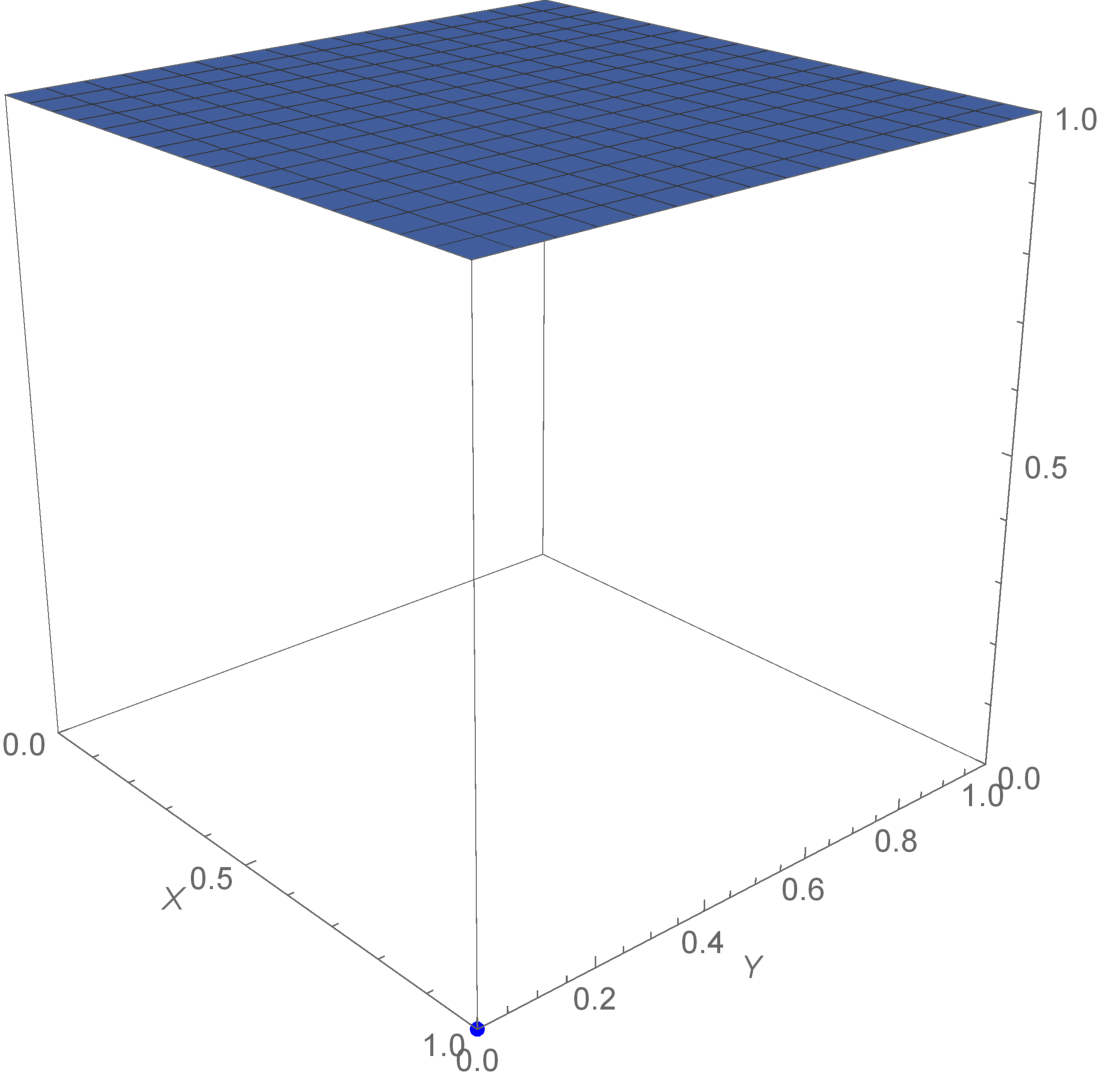
\includegraphics[width=4cm]{IGT.pdf} }
	\caption{Plots of basic fuzzy implication functions presented in Table \ref{table:basic_implications}.}\label{fig:basic_implications}
\end{figure}

\subsection{Families of fuzzy implication functions}\label{subsection:families}

In Table \ref{table:families_FI} we have provided an exhaustive list of families of fuzzy implication functions introduced in the literature and their respective construction methods. Thus, in this section we only take into account those families that are related to the results of this monograph. In particular, we recall the definition and motivation behind the definition of eleven families and we indicate the references in which studies of their additional properties can be found. Since this monograph is partially focused on the study of characterizations, we have recalled here the available characterizations of these families. Some of these characterizations are relatively recent and they are at the forefront of this research line.

\subsubsection{$(S,N)$ and $(U,N)$-implications}

In Section \ref{subsection:definition&additionalproperties} we comment that the generalization of classical tautologies to fuzzy logic is a common method for defining additional properties of fuzzy implication functions. This methodology has also been used as construction method for some families of fuzzy implication functions. For instance, the $S$-implications were introduced in \cite{Trillas1985} as the immediate generalization of the classical Boolean material implication $p \to q \equiv \neg p \vee q$, where the binary disjunction  $\vee $ was modeled by means of a t-conorm and the classical negation $\neg$ was modeled through a strong fuzzy negation $N$. In later studies, this family was generalized to $(S,N)$-implications by considering any fuzzy negation.

\begin{definition}[\textbf{\cite{Trillas1985,Dubois1991,Fodor1994,Klir1995}}]\label{def:(S,N)}
	A function $I:[0,1]^2 \to [0,1]$ is called an \emph{$(S,N)$-implication} if there exist a t-conorm $S$ and a fuzzy negation $N$ such that
	$$I(x,y)=S(N(x),y), \quad x,y \in [0,1].$$
	If $I$ is an $(S,N)$-implication generated from $S$ and $N$, then it is denoted by $I_{S,N}$.
\end{definition}
Since this family of fuzzy implication functions is one of the most important families, a problem of interest throughout the last decades has been to provide a characterization in terms of their properties. Indeed, in \cite{Trillas1985} the authors already provided a characterization for $S$-implications.
\begin{theorem}[\bf{\cite[Theorem 3.2]{Trillas1985}}] 
	Let $I:[0,1]^2\to[0,1]$ be a fuzzy implication function. The following statements are equivalent:
	\begin{enumerate}[label=(\roman*)]
		\item $I$ is an $(S,N)$-implication generated from a continuous t-conorm $S$ and a strong negation $N$.
		\item $I$ satisfies {\bf (NP)}, {\bf (EP)} and {\bf (CP($N$))}.
	\end{enumerate}
\end{theorem}
Later, the authors in \cite{Baczynski2007} provided the characterization of $(S,N)$-implications when $N$ is a continuous negation.
\begin{theorem}[\textbf{\cite[Theorem 5.2]{Baczynski2007}}]\label{th:charac_(S,N)_Ncont}
	For a function $I : [0,1]^2 \to [0,1]$ the following statements are equivalent:
	\begin{enumerate}[label=(\roman*)]
		\item I is an $(S,N)$-implication generated by a t-conorm $S$ and a continuous fuzzy negation $N$.
		\item I satisfies \Ione, \EP and $N_I$ is a continuous fuzzy negation.
	\end{enumerate}	
	Moreover, the representation of the $(S,N)$-implication	 is unique with
	$$N(x)=N_I(x), \quad x \in [0,1],$$
	$$S(x,y)=I(\mathfrak{R}_N(x),y), \quad x,y \in [0,1].$$	
\end{theorem}

However, the characterization of $(S,N)$-implications where $N$ is a non-continuous negation remains an open problem \cite{Baczynski2013,Baczynski2007,Kacprzyk2015}. In Chapter \ref{chapter:chsnimplications} we further discuss this problem.

More generally, in \cite{Pradera2016} the authors study the family of fuzzy implication functions obtained by substituting the role of the classical disjunction in the material implication by any fuzzy disjunction $A$, resulting in the so-called $(A,N)$-implications. Apart from providing a unified view of all the generalizations of $(S,N)$-implications gathered in Table \ref{table:families_FI}, they derive some interesting conclusions. For instance, they prove that there is a one-to-one correspondence between fuzzy implication functions and disjunctors (see \cite[Theorem 40]{Pradera2016}). This result underscores the importance of this construction method. Nonetheless, the most well-known generalization of $(S,N)$-implications is when the t-conorm $S$ is substituted by a disjunctive uninorm, obtaining the family of $(U,N)$-implications.
\begin{definition}[\textbf{\cite[Definition 5.1]{Backzynski2009}}]\label{def:(U,N)}
	A function $I:[0,1]^2 \to [0,1]$ is called a \emph{$(U,N)$-operation} if there exist a uninorm $U$ and a fuzzy negation $N$ such that
	$$I(x,y)=U(N(x),y), \quad x,y \in [0,1].$$
	If $I$ is a $(U,N)$-operation generated from $U$ and $N$, then it is denoted by $I_{U,N}$.
\end{definition}

However, $(U,N)$-operations are fuzzy implication functions only when $U$ is a disjunctive uninorm (see \cite[Theorem 5.3]{Backzynski2009}). Only in this case, we say that $I_{U,N}$ is a $(U,N)$-implication. This family is also characterized only in the case when $N$ is a continuous fuzzy negation (see \cite[Theorem 6.5]{Backzynski2009}).

A study of the additional properties of $(S,N)$ and $(U,N)$-implications can be found in Sections 2.4 and 5.3 of \cite{Baczynski2008}.

% R and RU-implications
%\begin{center}
%	\textsc{$R$ and $RU$-implications}
%\end{center}

\subsubsection{$R$ and $RU$-implications}

Similarly to the introduction of $(S,N)$-implications, $R$-implications were also defined as the generalization of a classical concept. In this case, the focus is on the following identity of crisp set theory:
$$A^c \cup B = (A \setminus B)^c = \bigcup \{C \subseteq X \mid A \cap C \subseteq B\},$$
where $A$ and $B$ are subsets of some universal set $X$. This identity corresponds to an alternative way of defining Boolean implications which is used in intuitionistic logic. The family of $R$-implications generalizes this concept to fuzzy logic.
\begin{definition}[\textbf{\cite{Trillas1985,Dubois1991,Fodor1994,Klir1995}}]\label{def:rimplications}
	A function $I:[0,1]^2 \to [0,1]$ is called an \emph{$R$-implication} if there exists a t-norm $T$ such that
	\begin{equation}\label{eq:rimplications}
	I(x,y)=\sup \{t \in [0,1] \mid T(x,t) \leq y\}, \quad x,y \in [0,1].
	\end{equation}
	If $I$ is an $R$-implication generated from a t-norm $T$, then it is denoted by $I_T$.
\end{definition}
The name of ``$R$-implication'' comes from a very important property related to this family, called the residuation property. However, this property is only satisfied when $T$ is a left-continuous t-norm.
\begin{proposition}[\bf{\cite[Proposition 2.5.2]{Baczynski2008}}]\label{prop:rimpl:residualproperty}
	For a t-norm $T$ the following statements are equivalent:
	\begin{enumerate}[label=(\roman*)]
		\item $T$ is left-continuous.
		\item $T$ and $I_T$ form an adjoint pair, i.e., they satisfy the following residual principle
		$$T(x,z) \leq y \Leftrightarrow I_T(x,y) \geq z, \quad x,y,z\in[0,1]. \eqno {\text{\RP}}$$
		\item The supremum in Equation (\ref{eq:rimplications}) is the maximum, i.e.,
		$$I_T(x,y)=\max \{t \in [0,1] \mid T(x,t) \leq y\}, \quad x,y \in [0,1].$$
	\end{enumerate}
\end{proposition}
The residuation property in Proposition \ref{prop:rimpl:residualproperty} strictly relates the structure of left-continuous t-norms and $R$-implications (see \cite{Jenei1998}). Moreover, in the case of left-continuous t-norms there is also a characterization of $R$-implications.
\begin{theorem}[\bf{\cite{Miyakoshi1985,Fodor1994}}]
	For a function $I:[0,1]^2 \to [0,1]$ the following statements are equivalent:
	\begin{enumerate}[label=(\roman*)]
		\item $I$ is an $R$-implication generated from a left-continuous t-norm.
		\item $I$ satisfies \Itwo, \EP, \OP and it is right-continuous with respect to the second variable.
	\end{enumerate}
\end{theorem}

For the family of $R$-implications there are also several generalizations, which are based on substituting the t-norm by another fuzzy operator. In fact, in \cite{Ouyang2012} the general case in which the role of the t-norm in Definition \ref{def:rimplications} is taken by any binary operator was considered. However, similarly to the case of $(A,N)$-operators, the most well-known generalization of $R$-implications is the one that considers uninorms.

\begin{definition}[\bf{\cite[Definition 5.4.1]{Baczynski2008}}]\label{def:ruoperations}
	A function $I:[0,1]^2 \to [0,1]$ is called an \emph{$RU$-operation} if there exists a uninorm $U$ such that
	$$I(x,y) = \sup \{t \in [0,1] \mid U(x,t) \leq y\}, \quad x,y \in [0,1].$$
	If $I$ is an $RU$-operation generated from a uninorm $U$, then it is denoted by $I_U$.
\end{definition}

Similarly to $(U,N)$-operators, only when $I_U$ is a fuzzy implication function we use the term $RU$-implication. See \cite[Corollary 5.4.4]{Baczynski2008} for some classes of uninorms in which this condition holds. The characterization of $RU$-implications for left-continuous uninorms is also available \cite{Aguilo2010}.

A study of the additional properties of $R$ and $RU$-implications can be found in Sections 2.5 and 5.4 of \cite{Baczynski2008}.

\subsubsection{$QL$ and $D$-implications}
The family of $QL$-implications was introduced as the generalization of the following implication defined in quantum logic: $p \to q \equiv \neg p \vee ( p \wedge q)$.
\begin{definition}[\textbf{\cite[Definition 4]{Mas2006}}]\label{def:QLimplications}
	A function $I:[0,1]^2 \to [0,1]$ is called a \emph{$QL$-operation} if there exist a t-norm $T$, a t-conorm $S$ and a fuzzy negation $N$ such that
	$$I(x,y)=S(N(x),T(x,y)), \quad x,y \in [0,1].$$
	If $I$ is a $QL$-operation generated from the triple $(T,S,N)$, then it is denoted by $I_{T,S,N}$.
\end{definition}
On the other hand, $D$-implications come from the Dishkant arrow: $p \to q \equiv (\neg p \wedge \neg q)\vee q$. 
\begin{definition}[\textbf{\cite[Definition 4]{Mas2006}}]
	A function $I : [0,1]^2 \to [0,1]$ is called a \emph{$D$-operation} if there exist a t-norm $T$, a t-conorm $S$ and a fuzzy negation $N$ such that
	$$I(x,y)=S(T(N(x),N(y)),y), \quad x,y \in [0,1].$$
	If $I$ is a $D$-operation generated from the triple $(S,T,N)$, then is denoted by $I_{S,T,N}$.
\end{definition}

Only when $I_{T,S,N}$ (resp. $I_{S,T,N}$) is a fuzzy implication function we use the term $QL$-implication (resp. $D$-implication). However, unlike other families, there is not an available characterization of those $QL$ or $D$-operators that are fuzzy implication functions, only some partial results are known \cite{Mas2006}. Also, there is no characterization available of these two families, although the characterization of a subclass of $QL$-implications can be found in \cite{Shi2008}.

A study of the additional properties of these two families can be found in \cite[Section 2.6]{Baczynski2008} and \cite{Trillas2000,Trillas2005,Mas2006}.

\subsubsection{Yager's $f$ and $g$-generated, $h$ and $k$-implications}

%% Yager's Implications & h-implications %%
Among those fuzzy implication functions whose definition is based on the use of generator functions, we can highlight Yager's implications, called $f$ and $g$-generated implications. These fuzzy implication functions are generated from additive generators of continuous Archimedean t-norms and t-conorms, respectively.

\begin{definition}[\bf{\cite{Yager2004}}]\label{def:fimpl} 
	Let $f:[0,1] \to [0,+\infty]$ be a strictly decreasing and continuous function with $f(1)=0$. The function $I_f:[0,1]^2 \to [0,1]$ defined by
	$$ I_f(x,y)=f^{-1}(x \cdot f(y)), \quad x,y \in [0,1],$$
	with the understanding $0 \cdot (+ \infty) = 0$, is called an \emph{$f$-generated implication}. The function $f$ itself is called an \emph{$f$-generator}.
	\label{yager_f}
\end{definition}
\begin{definition}[\bf{\cite{Yager2004}}]\label{def:gimpl} 
	Let $g:[0,1] \to [0,+\infty]$ be a strictly increasing and continuous function with $g(0)=0$. The function $I_g:[0,1]^2 \to [0,1]$ defined by
	$$I_g(x,y)=g^{(-1)}\left(\frac{1}{x}\cdot g(y)\right), \quad x,y \in [0,1],$$
	with the understanding $\frac{1}{0}=+\infty$ and $+\infty \cdot 0 = +\infty$ and where the function $g^{(-1)}$ is the pseudo-inverse of $g$ given by
	$$g^{(-1)}(x)=\left \{\begin{array}{ll} g^{-1}(x)& \hbox{if } x \in [0,g(1)],\\ 1&\hbox{if } x \in [g(1),+\infty],\end{array}\right.$$
	 is called a \emph{g-generated implication}. The function $g$ itself is called a \emph{$g$-generator}.
	\label{yager_g}
\end{definition}

In \cite{Yager2004}, Yager gives an extensive analysis of the role of these new classes of implications in approximate reasoning. In particular, he introduces and studies some new interesting concepts like strictness of implications, sharpness of inference, or the strictness index. According to him, these new operators are interesting in approximate reasoning since they accomplish strictness of a fuzzy implication function and sharpness of inference.

The characterization of these two families remained an open problem for almost a decade since the introduction of these classes in \cite{Yager2004} in 2004. They were characterized in 2012 by using the law of importation as the key algebraical property \cite{Massanet2012B}.

\begin{theorem}[\bf{\cite[Theorem 6]{Massanet2012B}}] 
	\label{thm:Char_F_1}
	Let $I:[0,1]^2\to [0,1]$ be a binary function. Then the following statements are equivalent:
	\begin{enumerate}
		\item[(i)] $I$ is an $f$-generated implication with $f(0)<+\infty$.
		\item[(ii)] $I$ satisfies \LI with \TP and $N_I$ is a strict negation.
	\end{enumerate}
	Moreover, in this case the $f$-generator is unique up to a positive multiplicative constant and it is given by $f(x)=N_I^{-1}(x)$. 
\end{theorem}

\begin{theorem}[\bf{\cite[Theorem 12]{Massanet2012B}}] 
	\label{thm:Char_F_Inf}
	Let $I:[0,1]^2\to [0,1]$ be a binary function. Then the following statements are equivalent:
	\begin{enumerate}
		\item[(i)] $I$ is an $f$-generated implication with $f(0)=+\infty$.
		\item[(ii)] $I$ satisfies \LI with \TP, $I$ is continuous except at $(0,0)$ and $I(x,y)=1 \Leftrightarrow x=0 \hbox{ or } y=1$. 
	\end{enumerate}
\end{theorem}

\begin{theorem}[\bf{\cite[Theorem 17]{Massanet2012B}}] 
	\label{thm:Char_G_1}
	Let $I:[0,1]^2\to [0,1]$ be a binary function. Then the following statements are equivalent:
	\begin{enumerate}
		\item[(i)] $I$ is a $g$-generated implication with $g(1)<+\infty$.
		\item[(ii)] $I$ satisfies \LI with \TP and there exists a continuous and strictly increasing function $t:[0,1] \to [0,1]$ with $t(0)=0$ and $t(1)=1$ such that ($I(x,y) = 1 \Leftrightarrow y \geq t(x)$).
	\end{enumerate}
	Moreover, in this case the $g$-generator is unique up to a positive multiplicative constant and it is given by $g(x)=t^{-1}(x)$. 
\end{theorem}

\begin{theorem}[\bf{\cite[Theorem 14]{Massanet2012B}}] 
	\label{thm:Char_G_Inf}
	Let $I:[0,1]^2\to [0,1]$ be a binary function. Then the following statements are equivalent:
	\begin{enumerate}
		\item[(i)] $I$ is a $g$-generated implication with $g(1)=+\infty$.
		\item[(ii)] $I$ satisfies \LI with \TP, $I$ is continuous except at $(0,0)$ and ($I(x,y)=1 \Leftrightarrow x=0 \hbox{ or } y=1$). 
	\end{enumerate}
\end{theorem}

A study of the additional properties of these two families can be found in \cite[Chapter 3]{Baczynski2008}.


Another family of fuzzy implication functions of this kind are the $h$-implications, introduced in \cite{Massanet2011A} following the idea behind the definition of Yager's implications but considering additive generators of representable uninorms.
\begin{definition}[\textbf{\cite[Definition 7]{Massanet2011A}}]\label{Defhimpl} Fix an $e \in (0,1)$ and let $h:[0,1] \to [-\infty,+\infty]$ be a strictly increasing and continuous function with $h(0)=-\infty$, $h(e)=0$ and $h(1)=+\infty$. The function $I^h:[0,1]^2 \to [0,1]$ defined by
	$$I^h(x,y)=\left \{\begin{array}{ll} 1& \hbox{if } x=0,\\
		h^{-1}(x\cdot h(y))&\hbox{if } x>0 \hbox{ and } y \leq e, \\
		h^{-1}(\frac{1}{x}\cdot h(y))&\hbox{if } x>0 \hbox{ and } y > e,
	\end{array}\right.
	$$
	is called an \emph{$h$-implication}. The function $h$ itself is called an \emph{$h$-generator} (with respect to e) of the fuzzy implication function $I^h$ defined as above.
\end{definition}

This family was characterized in \cite{Massanet2012A}. Specifically, it was proved that the characterization of $h$-implications could be derived from the characterization of Yager's implications since the structure of an $h$-implication is given by an $f$ and a $g$-generated implication through the horizontal threshold generation method. The horizontal threshold generation method is a construction method that generates a fuzzy implication function from two given ones and it consists in an appropriate scaling of the second variable of the two fuzzy implication functions.

\begin{theorem}[\textbf{\cite[Theorem 3]{Massanet2012A}}] Let $I_1$, $I_2$ be two fuzzy implication functions and $e \in (0,1)$. Then the binary function $I_{I_1-I_2}:[0,1]^2 \to [0,1]$, called the \emph{$e$-horizontal threshold} generated implication from $I_1$ and $I_2$, defined as
	$$I_{I_1-I_2}(x,y)=\left \{\begin{array}{ll} 1& \hbox{if } x=0,\\
		e \cdot I_1\left(x,\frac{y}{e}\right) &\hbox{if } x>0 \hbox{ and } y \leq e, \\
		e+(1-e)\cdot I_2\left(x,\frac{y-e}{1-e}\right) &\hbox{if } x>0 \hbox{ and } y > e,
	\end{array}\right.
	$$
	is a fuzzy implication function.
	\label{horizontalthreshold}
\end{theorem}

\begin{theorem}[\textbf{\cite[Theorem 2]{Massanet2012A}}]\label{th:characterizationh}
	Let $I:[0,1]^2 \to [0,1]$ be a binary function and $e \in (0,1)$. Then $I$ is an $h$-implication with respect to $e$ if and only if there exist $f$ and $g$-generated implications with $f(0)=g(1)=+\infty$, $I_f$ and $I_g$ respectively, such that $I$ is given by $I=I_{I_f-I_g}$. Moreover, in this case generators $h$, $f$ and $g$ are related in the following way:
	$$f(x)=-h(ex), \quad g(x)=h(e+(1-e)x), \quad \text{for all } x \in [0,1],$$
	$$
	h(x)=\left \{\begin{array}{ll} -f \left(\frac{x}{e}\right)& \hbox{if } x \leq e,\\
		g \left(\frac{x-e}{1-e}\right)&\hbox{if } x>e.
	\end{array}\right.
	$$
\end{theorem}

A study of the additional properties of this family can be found in \cite{Massanet2011A} and \cite[Section 5]{Hlinena2013}.

Another of the families of fuzzy implication functions that we are particularly interested in this monograph is a Yager's related class introduced in 2021 \cite{Zhou2021}. In this paper, the author defines a new family of fuzzy implication functions generated by multiplicative generators of continuous Archimedean t-norms. 

\begin{definition}[\bf{\cite[Definition 8]{Zhou2021}}] 
	Let $k:[0,1]\to[0,1]$ be a strictly increasing and continuous function with $k(1)=1$. The function $I_k : [0,1]^2 \to [0,1]$ defined by
	$$I_k(x,y)=k^{(-1)}\left( \frac{1}{x} \cdot k(y)\right), \quad x,y\in[0,1],$$ 
	with the understanding $\frac{0}{0}=1$ and $\frac{1}{0}=+\infty$ and where $k^{(-1)}$ is the pseudo-inverse of $k$, is called a \emph{$k$-generated implication}. The function $k$ itself is called a \emph{$k$-generator}.
\end{definition}

In the same paper, the author studies several additional properties of this family and he provides the characterization of some subclasses (see \cite[Theorems 2, 5 and 6]{Zhou2021}).

A particularly interesting fact about this family is that, while it is unkown when Yager's implications satisfy \TC, $k$-implications satisfy this property in many cases.

\begin{proposition}[\bf{\cite[Proposition 11]{Zhou2021}}] 
	Let $k$ be a $k$-generator with $k\leq id_{[0,1]}$, $I_k$ the $k$-generated implication and $T_k$ the t-norm generated
	by $k$ as its multiplicative generator. Then, $I_k$ satisfies \TC with
	each t-norm $T$ that is weaker than $T_k$, i.e., $T\leq T_k$.
\end{proposition}

Indeed, in 	\cite[Example 4]{Zhou2021} several pairs of parametric fuzzy implication functions and t-norms that satisfy \TC are provided.

%\begin{center}
%	\textsc{Probabilistic Implications}
%\end{center}

\subsubsection{Probabilistic implications}

In \cite{Grzegorzewski2011,Grzegorzewski2012} new families of fuzzy implication functions with a very interesting and novel origin were introduced. These families  are based on copulas and their definition combines fuzzy concepts and probability theory. According to the author, these families of operators may be useful in situations when we have to cope with imperfect knowledge with both kinds of uncertainty: imprecision and randomness. In particular, four families were defined: probabilistic implications, survival implications, probabilistic $S$-implications and survival $S$-implications. However, in \cite{Massanet2017B} it is proved that the families of probabilistic $S$-implications and survival $S$-implications are equal and in \cite{Massanet2019D} that the families of probabilistic and survival implications are equal. These results were a major breakthrough in the field since from 2011 until 2019 they were studied as different families. This event emphasizes the importance of the study of intersections and characterizations of fuzzy implication functions.

With regard to the results of this monograph, we are interested in probabilistic implications. The idea beyond this family of fuzzy implication functions is first to interpret the probability of an implication as the conditional probability
$$ P(B \mid A) = \frac{P(A \cap B)}{P(A)},$$
and then use the Sklar's theorem to transform the problem into the unit square.

\begin{proposition}[\textbf{\cite[Definition 4 and Theorem 6]{Grzegorzewski2011}}] Let $C$ be a copula. The function $I_C: [0,1]^2 \to [0,1]$ given by
$$I_C(x,y)
=
\left \{\begin{array}{ll} 
	1& \hbox{if } x=0,\\
	\frac{C(x,y)}{x} &\hbox{if } x>0,
\end{array}\right.
$$
is a fuzzy implication function if and only if
$$C(x_1,y)x_2 \geq C(x_2,y)x_1, \quad \text{for all } x_1 \leq x_2 \text{ and } y \in [0,1].$$
In this case, $I_C$ is called a \emph{probabilistic implication} (based on the copula $C$).
\end{proposition}

A study of the additional properties of this family can be found in \cite{Grzegorzewski2011,Grzegorzewski2013,Baczynski2016}. Further, in \cite{Massanet2019D} a characterization of this family was provided.

\begin{theorem}[\textbf{\cite[Theorem 19]{Massanet2019D}}]
	Let $I: [0,1]^2 \to [0,1]$ be a binary function. The following statements are equivalent:
	\begin{enumerate}[label=(\roman*)]
		\item $I$ is a probabilistic implication derived from a copula $C$.
		\item $N_I=\NDOne$ and $I$ satisfies \Ione, \NP, ($I(0,y)=1$ for all $y \in [0,1]$) and
		$$x_2I(x_2,y_1)+x_1I(x_1,y_2) \leq x_1I(x_1,y_1)+x_2I(x_2,y_2),$$
		for all $x_1 \leq x_2$ and $y_1 \leq y_2$.
	\end{enumerate}
\end{theorem}

%% Power-based implications %%

%\begin{center}
%	\textsc{Power-based Implications}
%\end{center}

\subsubsection{Power-based implications}

In Section \ref{subsection:definition&additionalproperties} we define the $T$-power invariance with respect to continuous t-norms \PIT, a property which is relatively novel since it was introduced in 2017 \cite{Massanet2017}. In this same paper, the authors point out that the main families of fuzzy implication functions do not fulfill this property. In this context, they presented $T$-power based implications as a family of fuzzy implication functions defined by a continuous t-norm $T$ and fulfilling the invariance for many choices of $T$ (see \cite{Massanet2017} and its corrigendum \cite{Massanet2019}). 

\begin{definition}[\textbf{\cite[Definition 4]{Massanet2017}}]
	A binary operator $I:[0,1]^2\to[0,1]$ is said to be a \emph{$T$-power based implication} if there exists a continuous t-norm $T$ such that 
	\[
	I(x,y)=\sup \{r \in [0,1] \ | \ y_T^{(r)} \geq x \}\qquad \hbox{for all } \  x, y \in [0,1].
	\]
	If $I$ is a $T$-power based implication, then it is denoted by $I^T$.
\end{definition}
In particular, the structure of $T$-power based implications when is a $T$ continuous Archimedean t-norm is provided by the following proposition.
\begin{proposition}[\bf{\cite[Proposition 5]{Massanet2017}}] Let $T$ be a continuous Archimedean t-norm and $t$ an additive generator of $T$. Then, its power based implication $I^T$ is defined as follows
	$$
	I^T(x,y)
	=
	\left\{ \begin{array}{ll}
		1 &  \text{if }  x \leq y, \\[3pt]
		\frac{t(x)}{t(y)} & \text{if }  x>y,
	\end{array}
	\right.
	$$
	with the convention that $\frac{a}{+\infty}=0$ for all $a \in [0,1]$.
\end{proposition}

A study of the additional properties of this family can be found in \cite{Massanet2017,Massanet2019B,Li2022,Li2023,Peng2022B,Peng2022}. Also, characterizations of this family were presented in \cite{Massanet2019B}, let us recall the corresponding results in the case of continuous Archimedean t-norms.

\begin{proposition}[\bf{\cite[Proposition 17]{Massanet2019B}}]
	Let $I: [0,1]^2 \to [0,1]$ be a binary function. Then $I$ is a $T$-power based implication for some nilpotent t-norm $T$ if and only if the following properties hold:
	\begin{enumerate}[label=(\roman*)]
		\item $I$ satisfies \OP;
		\item $I(x,y) \cdot I(y,0)=I(x,0)$ for all $x>y$;
		\item $I(\cdot,0)$ is a continuous, strictly decreasing function with $I(1,0)=0$.
	\end{enumerate}
	Moreover, in this case the t-norm $T$ is the nilpotent Archimedean t-norm with additive generator $t(x)=I(x,0)$ for all $x \in [0,1]$.
\end{proposition}

\begin{proposition}[\bf{\cite[Proposition 18]{Massanet2019B}}]
	Let $I: [0,1]^2 \to [0,1]$ be a binary function. Then $I$ is a $T$-power based implication for some strict t-norm $T$ if and only if $I$ satisfies \OP and there exists $k \in (0,1]$ such that the following properties hold:
	\begin{enumerate}[label=(\roman*)]
		\item $I(x,y) \cdot I(y,z) = I(x,z)$ for all $x>y>z>0$ and $z<k$;
		\item $\varphi_z : (z,1] \to [0,1]$ defined by $\varphi_z(x)=I(x,z)$ is a continuous, strictly decreasing function for all $0<z<k$;
		\item $I(x,0)=0$ for all $x>0$;
		\item $I(1,y)=0$ for all $y<1$;
		\item $\displaystyle I(x,0)=\lim_{y \to 0^+}I(x,y)$.
	\end{enumerate}
\end{proposition}









 